\clearpage
\section{Experimental Details}
\label{app:details}

% Compact appendix float helpers. The main preamble should load booktabs,
% graphicx, multirow, and ideally placeins. If placeins is not loaded,
% the following fallback prevents \FloatBarrier from breaking compilation.
\providecommand{\FloatBarrier}{}
\providecommand{\appCompactTable}[1]{%
  \begingroup
  \scriptsize
  \setlength{\tabcolsep}{3pt}%
  \renewcommand{\arraystretch}{0.95}%
  \resizebox{\columnwidth}{!}{#1}%
  \endgroup
}
\providecommand{\appWideTable}[1]{%
  \begingroup
  \scriptsize
  \setlength{\tabcolsep}{4pt}%
  \renewcommand{\arraystretch}{0.95}%
  \resizebox{\textwidth}{!}{#1}%
  \endgroup
}

% Tighter float spacing to reduce gaps between consecutive tables in the appendix.
\setlength{\textfloatsep}{8pt plus 2pt minus 2pt}
\setlength{\intextsep}{6pt plus 2pt minus 2pt}
\setlength{\floatsep}{6pt plus 2pt minus 2pt}
\setlength{\dbltextfloatsep}{8pt plus 2pt minus 2pt}
\setlength{\dblfloatsep}{6pt plus 2pt minus 2pt}

\subsection{Model and Fine-Tuning Configuration}
\label{app:models}

\begin{figure*}[t]
  \centering
  \includegraphics[
    width=0.99\textwidth,
    height=0.5\textheight,
    keepaspectratio
  ]{figures/dark_sub_overview.png}
    \caption{
    SAE training and evaluation pipeline for fine-tuned LLM activations.
    Only the member subset $D_{\mathrm{mem}}$ is used to fine-tune the pretrained open-weights LLM.
    The fine-tuned model is then evaluated on $D_{\mathrm{mem}}$, $D_{\mathrm{non}}$, and $D_{\mathrm{disjoint}}$ to extract layer-$\ell$ activations
    $H=\{h_{\mathrm{mem}},h_{\mathrm{non}},h_{\mathrm{disjoint}}\}$, which train an overcomplete sparse autoencoder.
    At evaluation time, the SAE reconstructs only member and non-member activations, yielding $\hat{h}_{\mathrm{mem}}$ and $\hat{h}_{\mathrm{non}}$.
    }
  \label{fig:dark-sub-overview}
\end{figure*}

\begin{table}[!htbp]
\centering
\caption{Models, fine-tuning configurations, and sparse autoencoder specifications.
All fine-tuning uses the AdamW optimizer with a cosine learning rate schedule and a maximum learning rate of $2 \times 10^{-5}$.}
\label{tab:model_details}
\appCompactTable{\begin{tabular}{@{}llcccc@{}}
\toprule
\textbf{Model} & \textbf{Architecture} & \textbf{Params} & \textbf{SAE layer} & \textbf{Dict.\ size} & \textbf{CF count} \\
\midrule
Pythia-1B      & GPT-NeoX  & 1.0B & 8  & 16{,}384  & 4  \\
Pythia-6.9B    & GPT-NeoX  & 6.9B & 16 & 32{,}768  & 131 \\
Pythia-12B     & GPT-NeoX  & 12B  & 24 & 20{,}480  & 9  \\
GPT-Neo-2.7B   & GPT-Neo   & 2.7B & 16 & 10{,}240  & 954 \\
OPT-6.7B       & OPT       & 6.7B & 24 & 32{,}768  & 55  \\
Falcon-7B      & Falcon     & 7.0B & 16 & 18{,}176  & 7  \\
Mistral-7B     & Mistral    & 7.2B & 16 & 16{,}384  & 10  \\
Llama-3-8B     & LLaMA      & 8.0B & 16 & 16{,}384  & ---  \\
Qwen2-7B       & Qwen2      & 7.6B & 16 & 14{,}336  & 7  \\
\bottomrule
\end{tabular}}
\end{table}

For Falcon-7B, 7 classifier features are identified pre-FDR and 0 survive Benjamini--Hochberg correction. FSC values are computed using the pre-FDR features.
Llama-3-8B is excluded from classifier-feature analyses because the available SAE checkpoint fails the reconstruction-quality criterion.
For Mistral-7B, 73 classifier features are identified pre-FDR and 10 survive Benjamini--Hochberg correction. FSC values use the pre-FDR features.
For Qwen2-7B, 15 classifier features are identified pre-FDR and 7 survive Benjamini--Hochberg correction.

Fine-tuned model weights are stored locally and loaded via the HuggingFace model loading interface.
All inference is conducted in half precision (float16) on NVIDIA A40, L40S, or H100 GPUs.
Sparse autoencoders are trained following the protocol of \citet{templeton2024scaling}, using an L1 penalty to encourage sparsity with 4$\times$ dictionary width.
Classifier features are identified by a two-sample test on activation magnitudes between members and non-members at a Benjamini--Hochberg corrected false discovery rate of 5\%.

\subsection{Channel Decomposition Details}
\label{app:bcd_details}

\paragraph{Contrastive principal component analysis.}
For each layer, we compute group covariance matrices on the mean-pooled hidden states.
The knowledge directions are the top eigenvectors of $\mathbf{C}_{\text{mem}} - \mathbf{C}_{\text{non}}$, and the recall directions are the top eigenvectors of $\mathbf{C}_{\text{hi}} - \mathbf{C}_{\text{lo}}$.
We retain $n_c = 10$ components for subspace construction and cosine analysis, and $n_c = 5$ for the erasure experiments in Appendix~\ref{app:dd_full}.
We verified that results are quantitatively stable for $n_c \in \{2, 3, 5, 10, 15, 20\}$. On Pythia-1B, $\cos(\dK, \dR)$ varies by less than 0.0002 across this range.

\paragraph{Recall label assignment.}
For each member text, we compute per-token cross-entropy loss and assign high-recall labels to members in the bottom 50\% of the loss distribution.
This proxy is validated by Spearman rank correlation with ROUGE-L extraction scores ranging from $\rho = -0.32$ to $\rho = -0.67$ across eight models (all $p < 10^{-24}$).
The negative sign reflects the convention that lower loss indicates higher recall.
Partial correlation on Pythia-6.9B controlling for loss shows that the recall direction $\dR$ retains a small but significant association with ROUGE-L ($\rho = +0.105$, $p = 0.001$), while the knowledge direction $\dK$ does not ($\rho = -0.037$, $p = 0.238$).

\paragraph{Probe training.}
Membership and recall probes are logistic regression classifiers trained on the projection of activations onto $\SK$ or $\SR$, respectively.
We report five-fold cross-validated AUROC.
Regularization strength is selected by nested cross-validation.

\subsection{Double Dissociation Protocol}
\label{app:dd_details}

For each model, we perform the intervention at the sparse autoencoder layer.
For each condition, we run the full forward pass with the modified activations and evaluate four metrics.
\begin{enumerate}
\item Detection AUROC using a loss-based detector, defined as member versus non-member classification based on per-token cross-entropy.
\item Mean member loss, defined as the average per-token cross-entropy over member texts. This acts as a proxy for recall disruption, where higher loss indicates that the model is less confident in reproducing the text.
\item ROUGE-L of greedy continuations from fixed-length prefixes, used as a direct measure of verbatim extraction.
\item Exact match rate, defined as the fraction of member texts whose greedy continuation matches the ground truth exactly.
\end{enumerate}
Erasure is applied at inference time only and does not modify model weights.

\paragraph{Subspace dimension and prefix length.}
The primary erasure experiments remove the leading $n_c = 10$ directions of the relevant subspace, matching the channel-decomposition rank used elsewhere in the paper. We also run an $n_c = 5$ sensitivity check whose full per-model metric tables appear in Appendix~\ref{app:dd_full}. The verbatim-extraction measurement uses ROUGE-L on greedy continuations from fixed-length prefixes, with prefixes truncated to a common length across all models so that prefix exposure is held constant when comparing extraction outcomes across the erasure conditions. The two ranks therefore probe whether the dissociation is robust to a halved subspace dimension while keeping the rest of the protocol fixed.

\subsection{Feature Ablation Protocol}
\label{app:ablation_details}

For the $k$-sweep experiment, we rank classifier features by the magnitude of their mean activation difference between members and non-members.
We then zero out the top-$k$ features in the sparse autoencoder encoding, decode back to the hidden-state space, and continue the forward pass.
We sweep $k$ from 1 to the total number of classifier features and measure both detection AUROC and extractability, using exact match rate and ROUGE-L.

\subsection{Scaling Curve}
\label{app:scaling}

\begin{table}[!htbp]
\centering
\caption{Scaling curve of membership detection across seven Pythia model sizes.
All models are fine-tuned under the same protocol on the same data.
$\mathrm{score}_K$ measures AUROC for projection onto the knowledge direction $\dK$.
Membership geometry is absent at 70M parameters and emerges above approximately 400M parameters (Figure~\ref{fig:arch_and_scaling}, right).}
\label{tab:scaling}
\appCompactTable{\begin{tabular}{@{}lc@{}}
\toprule
\textbf{Model} & \textbf{$\mathrm{score}_K$ AUROC} \\
\midrule
Pythia-70M   & 0.507 \\
Pythia-160M  & 0.588 \\
Pythia-410M  & 0.716 \\
Pythia-1B    & 0.800 \\
Pythia-2.8B  & 0.842 \\
Pythia-6.9B  & 0.876 \\
Pythia-12B   & 0.781 \\
\bottomrule
\end{tabular}}
\end{table}

To characterize when the membership geometry appears, we fine-tune seven Pythia models from 70M to 12B parameters under the same protocol and measure $\mathrm{score}_K$ at each scale (Table~\ref{tab:scaling}, Figure~\ref{fig:arch_and_scaling} right).
At 70M parameters, membership detection is at chance (0.507).
The signal rises steadily through 160M (0.588) and 410M (0.716), reaching above 0.80 at 1B parameters, with the strongest detection at 6.9B (0.876).
We interpret the transition between 160M and 410M as an approximate emergence threshold.

Pythia-12B breaks the monotonic trend, dropping to 0.781 after peaking at 6.9B.
This dip likely reflects a layer-selection artifact. At layer 18, the channel decomposition detects a $\mathrm{score}_K$ of 0.766, and both layers show the same reconstruction/residual pattern (16pp drop at layer 18 versus 14pp at layer 24).

\FloatBarrier

\section{Additional Results}
\label{app:additional}

\subsection{Per-Layer Decomposition Tables}
\label{app:per_layer}

Tables~\ref{tab:p1b_layers}--\ref{tab:qwen2_layers} provide the full per-layer channel decomposition results for each model, including GPT-Neo-2.7B (Table~\ref{tab:neo_layers}).

\begin{table}[!htbp]
\centering
\caption{Per-layer channel decomposition for Pythia-1B (epoch 5).}
\label{tab:p1b_layers}
\appCompactTable{\begin{tabular}{@{}ccccc@{}}
\toprule
\textbf{Layer} & $\cos(\dK, \dR)$ & \textbf{Angle ($\degree$)} & \textbf{Mem.\ AUROC} & \textbf{Rec.\ AUROC} \\
\midrule
0 & $-$0.170 & 20.3 & 0.487 & 0.660 \\
2 & $-$0.072 & 15.1 & 0.514 & 0.714 \\
4 & $-$0.082 & 12.7 & 0.510 & 0.737 \\
6 & $-$0.038 & 17.6 & 0.524 & 0.749 \\
8 & 0.102 & 16.7 & 0.577 & 0.762 \\
10 & 0.279 & 21.5 & 0.686 & 0.767 \\
12 & 0.402 & 20.8 & 0.739 & 0.744 \\
14 & 0.643 & 23.8 & 0.800 & 0.761 \\
15 & 0.671 & 25.5 & 0.771 & 0.746 \\
\bottomrule
\end{tabular}}
\end{table}

\begin{table}[!htbp]
\centering
\caption{Per-layer channel decomposition for Pythia-6.9B.}
\label{tab:p69_layers}
\appCompactTable{\begin{tabular}{@{}ccccc@{}}
\toprule
\textbf{Layer} & $\cos(\dK, \dR)$ & \textbf{Angle ($\degree$)} & \textbf{Mem.\ AUROC} & \textbf{Rec.\ AUROC} \\
\midrule
0 & $-$0.083 & 21.0 & 0.489 & 0.622 \\
4 & $-$0.013 & 14.9 & 0.492 & 0.750 \\
8 & 0.026 & 17.2 & 0.525 & 0.751 \\
12 & $-$0.008 & 20.4 & 0.689 & 0.728 \\
16 & 0.107 & 21.1 & 0.828 & 0.696 \\
20 & 0.109 & 21.6 & 0.876 & 0.686 \\
24 & 0.086 & 26.0 & 0.861 & 0.658 \\
28 & 0.056 & 26.6 & 0.860 & 0.663 \\
31 & 0.038 & 29.5 & 0.864 & 0.672 \\
\bottomrule
\end{tabular}}
\end{table}

\begin{table}[!htbp]
\centering
\caption{Per-layer channel decomposition for Pythia-12B.}
\label{tab:p12b_layers}
\appCompactTable{\begin{tabular}{@{}ccccc@{}}
\toprule
\textbf{Layer} & $\cos(\dK, \dR)$ & \textbf{Angle ($\degree$)} & \textbf{Mem.\ AUROC} & \textbf{Rec.\ AUROC} \\
\midrule
0  & $-$0.063 & 21.9 & 0.488 & 0.684 \\
6  & $-$0.060 & 14.8 & 0.513 & 0.767 \\
12 & 0.145 & 21.8 & 0.574 & 0.803 \\
18 & 0.255 & 21.2 & 0.741 & 0.820 \\
24 & 0.336 & 24.1 & 0.781 & 0.806 \\
30 & 0.540 & 26.2 & 0.742 & 0.808 \\
35 & 0.695 & 25.8 & 0.756 & 0.817 \\
\bottomrule
\end{tabular}}
\end{table}

\begin{table}[!htbp]
\centering
\caption{Per-layer channel decomposition for GPT-Neo-2.7B.}
\label{tab:neo_layers}
\appCompactTable{\begin{tabular}{@{}cccc@{}}
\toprule
\textbf{Layer} & $\cos(\dK, \dR)$ & \textbf{Mem.\ AUROC} & \textbf{Rec.\ AUROC} \\
\midrule
0 & $-$0.060 & 0.470 & 0.684 \\
4 & $-$0.001 & 0.493 & 0.691 \\
8 & 0.022 & 0.503 & 0.741 \\
12 & $-$0.119 & 0.497 & 0.815 \\
16 & 0.024 & 0.504 & 0.813 \\
20 & 0.140 & 0.486 & 0.805 \\
24 & 0.241 & 0.526 & 0.790 \\
28 & 0.245 & 0.521 & 0.788 \\
31 & 0.078 & 0.539 & 0.769 \\
\bottomrule
\end{tabular}}
\end{table}

\begin{table}[!htbp]
\centering
\caption{Per-layer channel decomposition for OPT-6.7B.}
\label{tab:opt_layers}
\appCompactTable{\begin{tabular}{@{}ccccc@{}}
\toprule
\textbf{Layer} & $\cos(\dK, \dR)$ & \textbf{Angle ($\degree$)} & \textbf{Mem.\ AUROC} & \textbf{Rec.\ AUROC} \\
\midrule
0 & $-$0.103 & 19.9 & 0.500 & 0.728 \\
4 & 0.382 & 20.2 & 0.499 & 0.819 \\
8 & 0.183 & 15.9 & 0.495 & 0.837 \\
12 & 0.121 & 20.7 & 0.514 & 0.843 \\
16 & 0.156 & 23.6 & 0.548 & 0.866 \\
20 & 0.183 & 25.8 & 0.753 & 0.880 \\
24 & $-$0.063 & 28.4 & 0.869 & 0.883 \\
28 & 0.029 & 31.1 & 0.848 & 0.879 \\
31 & 0.196 & 29.1 & 0.820 & 0.881 \\
\bottomrule
\end{tabular}}
\end{table}

\begin{table}[!htbp]
\centering
\caption{Per-layer channel decomposition for Falcon-7B.}
\label{tab:falcon_layers}
\appCompactTable{\begin{tabular}{@{}ccccc@{}}
\toprule
\textbf{Layer} & $\cos(\dK, \dR)$ & \textbf{Angle ($\degree$)} & \textbf{Mem.\ AUROC} & \textbf{Rec.\ AUROC} \\
\midrule
0 & $-$0.191 & 19.3 & 0.489 & 0.760 \\
4 & $-$0.062 & 16.2 & 0.479 & 0.798 \\
8 & 0.046 & 15.7 & 0.500 & 0.826 \\
12 & 0.087 & 22.4 & 0.549 & 0.846 \\
16 & 0.161 & 23.4 & 0.635 & 0.855 \\
20 & 0.209 & 24.4 & 0.690 & 0.861 \\
24 & 0.277 & 26.0 & 0.811 & 0.862 \\
28 & 0.579 & 27.8 & 0.829 & 0.872 \\
31 & 0.590 & 26.4 & 0.971 & 0.898 \\
\bottomrule
\end{tabular}}
\end{table}

\begin{table}[!htbp]
\centering
\caption{Per-layer channel decomposition for Mistral-7B.}
\label{tab:mistral_layers}
\appCompactTable{\begin{tabular}{@{}ccccc@{}}
\toprule
\textbf{Layer} & $\cos(\dK, \dR)$ & \textbf{Angle ($\degree$)} & \textbf{Mem.\ AUROC} & \textbf{Rec.\ AUROC} \\
\midrule
0 & $-$0.274 & 18.7 & 0.500 & 0.500 \\
4 & $-$0.306 & 16.6 & 0.527 & 0.793 \\
8 & $-$0.270 & 25.0 & 0.759 & 0.787 \\
12 & $-$0.092 & 22.8 & 0.919 & 0.758 \\
16 & $-$0.010 & 25.3 & 0.967 & 0.714 \\
20 & 0.029 & 26.2 & 0.975 & 0.661 \\
24 & 0.011 & 30.8 & 0.977 & 0.623 \\
28 & $-$0.021 & 35.2 & 0.997 & 0.609 \\
31 & 0.029 & 28.5 & 1.000 & 0.609 \\
\bottomrule
\end{tabular}}
\end{table}

\begin{table}[!htbp]
\centering
\caption{Per-layer channel decomposition for Llama-3-8B.}
\label{tab:llama3_layers}
\appCompactTable{\begin{tabular}{@{}ccccc@{}}
\toprule
\textbf{Layer} & $\cos(\dK, \dR)$ & \textbf{Angle ($\degree$)} & \textbf{Mem.\ AUROC} & \textbf{Rec.\ AUROC} \\
\midrule
0 & $-$0.093 & 21.4 & 0.498 & 0.610 \\
4 & $-$0.053 & 15.7 & 0.541 & 0.764 \\
8 & 0.018 & 18.6 & 0.723 & 0.754 \\
12 & 0.090 & 19.5 & 0.908 & 0.756 \\
16 & 0.223 & 22.0 & 0.957 & 0.735 \\
20 & 0.295 & 25.2 & 0.948 & 0.719 \\
24 & 0.271 & 26.0 & 0.954 & 0.702 \\
28 & 0.234 & 27.3 & 0.980 & 0.671 \\
31 & 0.321 & 29.5 & 0.999 & 0.661 \\
\bottomrule
\end{tabular}}
\end{table}

\begin{table}[!htbp]
\centering
\caption{Per-layer channel decomposition for Qwen2-7B.}
\label{tab:qwen2_layers}
\appCompactTable{\begin{tabular}{@{}ccccc@{}}
\toprule
\textbf{Layer} & $\cos(\dK, \dR)$ & \textbf{Angle ($\degree$)} & \textbf{Mem.\ AUROC} & \textbf{Rec.\ AUROC} \\
\midrule
0 & 0.145 & 17.1 & 0.497 & 0.549 \\
4 & 0.218 & 16.0 & 0.509 & 0.758 \\
8 & 0.176 & 14.7 & 0.550 & 0.724 \\
12 & 0.199 & 15.5 & 0.620 & 0.717 \\
16 & 0.390 & 17.5 & 0.803 & 0.705 \\
20 & 0.439 & 16.1 & 0.941 & 0.700 \\
24 & 0.440 & 20.1 & 0.940 & 0.692 \\
27 & 0.479 & 27.2 & 1.000 & 0.666 \\
\bottomrule
\end{tabular}}
\end{table}

\FloatBarrier

\subsection{Non-Linear Probing Comparison}
\label{app:nonlinear}

\begin{table}[!htbp]
\centering
\caption{Non-linear probing comparison.
Mean AUROC gap is MLP minus linear across all analyzed layers.
Positive values indicate the MLP outperforms the linear probe. Negative values indicate the linear probe is better.
All gaps are below 5 percentage points.}
\label{tab:nonlinear}
\appCompactTable{\begin{tabular}{@{}lcccc@{}}
\toprule
\textbf{Model} & \textbf{Mean gap (mem.)} & \textbf{Mean gap (rec.)} & \textbf{Max gap (mem.)} & \textbf{Max gap (rec.)} \\
\midrule
Pythia-1B   & $-$0.013 & $+$0.016 & $+$0.014 & $+$0.028 \\
Pythia-6.9B & $-$0.023 & $-$0.021 & $+$0.012 & $-$0.002 \\
Pythia-12B  & $-$0.032 & $-$0.009 & $+$0.028 & $+$0.033 \\
GPT-Neo-2.7B& $+$0.007 & $+$0.010 & $+$0.025 & $+$0.031 \\
OPT-6.7B    & $-$0.007 & $-$0.011 & $+$0.037 & $+$0.021 \\
Falcon-7B   & $-$0.019 & $-$0.000 & $+$0.031 & $+$0.013 \\
Mistral-7B  & $-$0.015 & $-$0.010 & $+$0.004 & $+$0.025 \\
\bottomrule
\end{tabular}}
\end{table}

Table~\ref{tab:nonlinear} reports the AUROC gap between MLP probes (two hidden layers, 256 and 128 units, ReLU activations, 5-fold cross-validation) and linear probes across all analyzed layers.
In five of seven models, the linear probe achieves \emph{higher} mean membership AUROC than the MLP, likely because the MLP's additional parameters overfit the relatively small probe training set.
The largest positive gap (MLP better) is 0.037 for OPT-6.7B membership at a single layer. The largest negative gap (linear better) is $-$0.032 for Pythia-12B membership.
These results provide no evidence that the tested MLP probes recover substantially more membership or recall signal than the linear probes under this sample size and regularization regime.

\subsection{Cross-Architecture Transfer Details}
\label{app:transfer}

To assess whether the K/R subspaces reflect shared geometric structure across architectures, we compute principal angles between the $\SK$ subspaces (rank $k = 10$) of all model pairs with matching hidden dimension ($d = 4{,}096$).
Principal angles measure the best-case alignment between two subspaces after optimal rotation, providing a strict test of geometric similarity.

\paragraph{Computation.}
Let $\mathbf{Q}_a \in \mathbb{R}^{d \times r_a}$ and $\mathbf{Q}_b \in \mathbb{R}^{d \times r_b}$ be orthonormal bases for the knowledge subspaces $\mathcal{S}_{K}^{(a)}$ and $\mathcal{S}_{K}^{(b)}$ of two models with matching hidden dimension $d$. The principal angles $\theta_i$ are read off the singular values of the cross-basis matrix.
\begin{equation}
\sigma_i\!\left(\mathbf{Q}_a^\top \mathbf{Q}_b\right) = \cos(\theta_i).
\label{eq:principal_angles}
\end{equation}
Larger singular values correspond to smaller principal angles and stronger raw subspace alignment. The test asks whether the two knowledge subspaces overlap in the models' original hidden-state coordinates. It is therefore a strict coordinate-level comparison and does not test whether the same information could be brought into alignment after learning a cross-model map or rotation. We pick rank $k = 10$ to match the channel-decomposition rank used elsewhere, and we compute the singular values via standard SVD of $\mathbf{Q}_a^\top \mathbf{Q}_b$.

Principal angle analysis across three models with matching hidden dimension ($d = 4{,}096$, namely Pythia-6.9B, OPT-6.7B, and Llama-3-8B) shows no evidence that any model pair shares subspace geometry beyond chance.
The mean squared cosine of principal angles ranges from 0.0015 to 0.0025 across all three pairs, indistinguishable from the random baseline of $0.0025 \pm 0.0003$.
This provides no evidence of shared subspace geometry under the strict same-dimensional principal-angle comparison, even though all models show K/R separation.

\subsection{Cross-Architecture Measure Readings}
\label{app:cross_arch_readings}

We elaborate the intuitive reading of each cross-architecture measure summarized in \S\ref{sec:methods:transfer}.

The first measure asks whether two models put their knowledge subspaces in the same place. Principal angles compare the leading directions of $\mathcal{S}_{K}^{(a)}$ and $\mathcal{S}_{K}^{(b)}$ inside a shared ambient vector space, restricted to model pairs at matching hidden dimension ($d = 4{,}096$). Small angles indicate similar directions, while angles near $90^\circ$ indicate near orthogonality. The comparison is strictly coordinate-level and does not learn a cross-model map.

The second measure asks how spread out a model's member activations are. The participation ratio reads as an effective number of active dimensions, high when variance is distributed across many directions and low when it is concentrated in a few. It summarizes whether member activations occupy a broad distributed region of activation space or a more compressed low-dimensional subspace.

The third measure asks whether the membership signal lives inside that dominant subspace at all. The mean-difference vector $\Delta_{\mathrm{mem}}$ between member and non-member activations points along the direction that separates the average member document from the average non-member document. The cross-architecture concentration $C_k$ reports the fraction of $\Delta_{\mathrm{mem}}$ captured by the top-$k$ principal-component basis. Values near 1 mean the shift lies along the dominant directions of member variation. Values near 0 mean it lies on lower-variance or off-subspace directions.

\subsection{Double Dissociation Across Fine-Tuning Epochs}
\label{app:epoch_dd}

\begin{table}[!htbp]
\centering
\caption{Double dissociation for Pythia-1B at epochs 1, 3, and 5.
At epoch 1, baseline detection is weak and erasure effects are minimal.
By epoch 3, the knowledge subspace carries sufficient signal for erasure to produce measurable drops.
Extraction ROUGE-L collapses under erasure at all epochs.}
\label{tab:epoch_dd}
\appCompactTable{\begin{tabular}{@{}llcccc@{}}
\toprule
\textbf{Epoch} & \textbf{Metric} & \textbf{Baseline} & \textbf{Erase $\SK$} & \textbf{Erase $\SR$} & \textbf{Erase both} \\
\midrule
\multirow{2}{*}{1} & Det.\ AUROC & 0.677 & 0.594 & 0.596 & 0.502 \\
                    & ROUGE-L     & 0.150 & 0.066 & 0.076 & 0.037 \\
\midrule
\multirow{2}{*}{3} & Det.\ AUROC & 0.993 & 0.900 & 0.914 & 0.705 \\
                    & ROUGE-L     & 0.170 & 0.044 & 0.053 & 0.030 \\
\midrule
\multirow{2}{*}{5} & Det.\ AUROC & 1.000 & 0.984 & 0.987 & 0.900 \\
                    & ROUGE-L     & 0.208 & 0.035 & 0.034 & 0.023 \\
\bottomrule
\end{tabular}}
\end{table}

Table~\ref{tab:epoch_dd} shows the progression of double dissociation results as fine-tuning proceeds.
At epoch 1, baseline detection AUROC is 0.677, above chance but far from perfect, and subspace erasure reduces it to near chance (0.502 under combined erasure), consistent with a nascent but fragile knowledge signal.
By epoch 3, the knowledge subspace has strengthened considerably. Baseline detection reaches 0.993, and erasing $\SK$ reduces it to 0.900 while erasing $\SR$ reduces it to 0.914.
By epoch 5, the detection signal is strong enough that single-subspace erasure produces only modest drops, to 0.984 and 0.987, while combined erasure still reduces detection to 0.900.
Extraction ROUGE-L collapses under erasure at all epochs, showing that the intervened subspaces are important for verbatim reproduction even when the knowledge signal is still developing.

\subsection{Full Metrics for Double Dissociation}
\label{app:dd_full}

\begin{table}[!htbp]
\centering
\caption{Double dissociation with all metrics for all models at epoch 5.
Mean member loss quantifies generation disruption. Exact match rate provides a strict extraction measure complementary to ROUGE-L.}
\label{tab:dd_full}
\appCompactTable{\begin{tabular}{@{}lcccc@{}}
\toprule
\textbf{Model} & \textbf{Baseline} & \textbf{Erase $\SK$} & \textbf{Erase $\SR$} & \textbf{Erase both} \\
\midrule
\multicolumn{5}{@{}l}{\emph{Mean member loss}} \\
Pythia-1B   & 0.565 & 3.675 & 3.625 & 4.734 \\
Pythia-6.9B & 0.041 & 9.025 & 8.603 & 9.667 \\
Pythia-12B  & 0.364 & 19.136 & 18.772 & 20.729 \\
OPT-6.7B    & 0.412 & 2.121 & 2.083 & 2.251 \\
\midrule
\multicolumn{5}{@{}l}{\emph{Exact match rate}} \\
Pythia-1B   & 0.064 & 0.008 & 0.007 & 0.006 \\
Pythia-6.9B & 0.740 & 0.007 & 0.010 & 0.006 \\
Pythia-12B  & 0.120 & 0.000 & 0.000 & 0.000 \\
OPT-6.7B    & 0.111 & 0.018 & 0.020 & 0.019 \\
\bottomrule
\end{tabular}}
\end{table}

\subsection{Directional Steering Results}
\label{app:steering}

Directional steering experiments add $\alpha \cdot \hat{d}$ to the residual stream at the sparse autoencoder layer, sweeping $\alpha \in \{-5, -3, -2, -1, 0, 1, 2, 3, 5\}$ for both the knowledge direction $\dK$ and the recall direction $\dR$.
For both Pythia-1B and Pythia-6.9B, baseline detection is already near-perfect, so all steering conditions yield detection AUROC at or near 1.000 regardless of direction or magnitude.
For Pythia-1B, steering along $\dR$ produces a slightly larger modulation of exact-match extraction than steering along $\dK$. The exact-match rate drops from roughly six percent at $\alpha{=}0$ to roughly four percent at $|\alpha|{=}5$ for $\dR$, compared with a drop from six percent to five percent for $\dK$.
For Pythia-6.9B, both directions produce negligible changes in extraction, with exact-match rates remaining near 72 percent across all conditions, consistent with the model's stronger memorization making single-direction perturbations insufficient to disrupt recall.
The ceiling effect contrasts with the double dissociation results, where full subspace erasure (rank-5 projection) produces substantial disruption.
This difference is consistent with the knowledge and recall signals being distributed across multiple directions within each subspace rather than concentrated in a single dominant activation direction, although the near-ceiling detection baseline limits what single-direction steering can establish.

\FloatBarrier

\subsection{Feature Sufficiency Criterion Values}
\label{app:fsc}

The feature sufficiency criterion evaluates geometric sufficiency. We ask whether the selected SAE features span the activation channel they are meant to explain. If they do not, then a feature-level intervention has little reason to affect that channel. The criterion is therefore a geometric prerequisite for the causal-effectiveness test that follows.

\begin{table*}[!htbp]
\centering
\caption{Feature sufficiency criterion (FSC) for classifier features and the full SAE dictionary relative to $\SK$ and $\SR$.
Random Mean reports the mean FSC($\SK$) from 1{,}000 random subsets of size $|$CF$|$ drawn from the full dictionary.
Percentile gives the rank of the observed FSC within the random null distribution.
Llama-3-8B is excluded because the available SAE checkpoint fails the reconstruction-quality criterion.}
\label{tab:fsc_values}
\appWideTable{\begin{tabular}{@{}lcccccc@{}}
\toprule
\textbf{Model} & \textbf{$n_{\text{CF}}$} & \textbf{FSC($\SK$, CF)} & \textbf{Random Mean} & \textbf{Pctl.} & \textbf{FSC($\SK$, all)} & \textbf{FSC($\SR$, all)} \\
\midrule
Pythia-1B    & 4   & 0.029 & 0.003 & 99.9\% & 1.000 & 1.000 \\
Pythia-6.9B  & 131 & 0.082 & 0.030 & 97.4\% & 1.000 & 1.000 \\
Pythia-12B   & 9   & 0.024 & 0.004 & 99.3\% & 1.000 & 1.000 \\
GPT-Neo-2.7B & 954 & 0.069 & 0.253 & 0.0\%  & 1.000 & 1.000 \\
OPT-6.7B     & 55  & 0.154 & 0.017 & 100.0\% & 1.000 & 1.000 \\
Falcon-7B    & 7   & 0.066 & 0.011 & 100.0\% & 1.000 & 1.000 \\
Mistral-7B   & 73  & 0.062 & 0.051 & 97.3\% & 1.000 & 1.000 \\
Qwen2-7B     & 15  & 0.109 & 0.019 & 100.0\% & 1.000 & 1.000 \\
\bottomrule
\end{tabular}}
\end{table*}

\paragraph{Value-interpretation axes.}
The feature sufficiency criterion is bounded between 0 and 1 by construction. Values near 1 mean that the selected SAE features span most of the target channel, so a feature-level intervention that ablates those features can in principle remove most of the channel-aligned variation. Values near 0 mean that the channel mostly lies outside those feature directions, so a feature-level intervention has little geometric reason to affect the channel even when it succeeds at suppressing the targeted features. The criterion therefore separates geometric compatibility (whether the chosen feature directions even contain the target channel) from causal effectiveness (whether ablation actually changes the downstream outcome).

Using all decoder vectors gives FSC of 1.000 for both subspaces in all models (Table~\ref{tab:fsc_values}) when the decoder span contains the channel subspace. The informative comparison is therefore the selected classifier-feature subset, whose FSC remains low across models.
The low FSC values for classifier features (0.024--0.154) indicate that the subset of features identified by the statistical test captures only a small fraction of the channel-defined subspaces.
To assess whether this low coverage is expected with so few classifier features, we compare each model's observed FSC against 1{,}000 random feature subsets of matched size.
In seven of eight interpretable models, the observed FSC exceeds the 97th percentile of the random null, indicating that classifier features are more aligned with $\SK$ than random dictionary elements.
GPT-Neo-2.7B is the exception (observed FSC 0.069, random mean 0.253, percentile 0.0\%).
Its 954 classifier features produce lower coverage than random subsets of the same size, suggesting that the membership-correlated features in this model are not aligned with the knowledge subspace under this FSC test.

\subsection{Per-Model Channel-Decomposition Geometry}
\label{app:per_model_bcd}

\begin{figure}[tbp]
  \centering
  
\includegraphics[width=\linewidth]{figures/layer_trajectories.pdf}
  \caption{Layer-by-layer probe performance and subspace alignment across nine models.
  Membership detector area under the receiver operating characteristic curve (solid), recall probe area under the curve (dashed), and cosine similarity between $\dK$ and $\dR$ (dotted).
  Knowledge and recall signals develop at different layers.
  The subspace directions maintain low mutual alignment throughout, with cosine similarity rising in late layers only for models under capacity pressure (Pythia-1B, Pythia-12B).}
  \label{fig:layer_trajectories}
\end{figure}

\begin{table}[!htbp]
\centering
\caption{Channel decomposition at the sparse autoencoder layer for each model.
Cosine similarity between leading directions $\dK$ and $\dR$ and cross-validated probe area under the receiver operating characteristic curve.
Cosine similarity remains below 0.40 in all nine models, indicating low mutual alignment between the two subspaces.}
\label{tab:bcd_main}
\appCompactTable{\begin{tabular}{@{}lccc@{}}
\toprule
\textbf{Model} & $\cos(\dK, \dR)$ & \textbf{Mem.\ AUROC} & \textbf{Rec.\ AUROC} \\
\midrule
Pythia-1B (ep.\,5) & 0.102 & 0.577 & 0.762 \\
Pythia-6.9B        & 0.107 & 0.828 & 0.696 \\
Pythia-12B         & 0.336 & 0.781 & 0.806 \\
GPT-Neo-2.7B       & 0.024 & 0.504 & 0.813 \\
OPT-6.7B           & $-$0.063 & 0.869 & 0.883 \\
Falcon-7B          & 0.161 & 0.635 & 0.855 \\
Mistral-7B         & $-$0.010 & 0.967 & 0.714 \\
Llama-3-8B         & 0.223 & 0.957 & 0.735 \\
Qwen2-7B           & 0.390 & 0.803 & 0.705 \\
\bottomrule
\end{tabular}}
\end{table}

\begin{table}[!htbp]
\centering
\caption{Norm--direction decomposition of membership detection.
GPT-family models rely primarily on directional structure, with norm AUROC near chance, while LLaMA-family models combine magnitude and direction.
Norm AUROC is reported at the best layer per model. $\mathrm{score}_K$ is reported at the SAE layer per model.}
\label{tab:norm_direction}
\appCompactTable{\begin{tabular}{@{}lccc@{}}
\toprule
\textbf{Model} & \textbf{Norm AUROC} & \textbf{$\mathrm{score}_K$} & \textbf{$\mathrm{score}_K$ advantage} \\
\midrule
\multicolumn{4}{@{}l}{\emph{GPT-family}} \\
Pythia-6.9B    & 0.542 & 0.803 & +26\,pp \\
OPT-6.7B       & 0.534 & 0.774 & +24\,pp \\
Falcon-7B      & 0.557 & 0.690 & +13\,pp \\
Pythia-1B      & 0.548 & 0.660 & +11\,pp \\
Pythia-12B     & 0.599 & 0.707 & +11\,pp \\
GPT-Neo-2.7B   & 0.514 & 0.616 & +10\,pp \\
Qwen2-7B       & 0.542 & 0.638 & +10\,pp \\
\midrule
\multicolumn{4}{@{}l}{\emph{LLaMA-family}} \\
Mistral-7B     & 0.877 & 0.927 & +5\,pp \\
Llama-3-8B     & 0.843 & 0.903 & +6\,pp \\
\bottomrule
\end{tabular}}
\end{table}

This section provides model-specific commentary on the channel decomposition results summarized in Table~\ref{tab:bcd_main}.

\paragraph{Pythia models.}
In the two models with hidden dimension 4{,}096 (Pythia-6.9B and OPT-6.7B), cosine similarity remains below 0.11 at the sparse autoencoder layer.
Pythia-12B, the largest model in the Pythia family, shows cosine 0.336 at its sparse autoencoder layer.
This rises to 0.695 in the final layers, a pattern shared with Pythia-1B, suggesting that the GPT-NeoX architecture entangles the two signals in late layers.

\paragraph{OPT-6.7B.}
OPT-6.7B achieves a near-zero cosine ($-$0.063) paired with the highest recall AUROC (0.883), indicating that the two subspaces can both be high-quality and weakly aligned.

\paragraph{GPT-Neo-2.7B.}
GPT-Neo-2.7B shows near-zero cosine (0.024) with membership detection at chance (AUROC 0.504), showing that the membership signal has not consolidated at this layer and serving as a negative control.

\paragraph{Falcon-7B.}
Falcon-7B, from a distinct architecture family (multi-query attention, RefinedWeb pretraining), shows cosine 0.161 at its sparse autoencoder layer with the second-highest recall AUROC (0.855) after OPT-6.7B (0.883), providing cross-family evidence of low alignment between the two subspaces.

\paragraph{Mistral-7B.}
Mistral-7B shows the lowest absolute cosine ($-$0.010) and the strongest membership detection (AUROC 0.967) among all nine models, showing that minimal alignment between the two directions is compatible with highly discriminative knowledge representations.
The negative sign indicates a slight anti-alignment between the leading directions, further supporting the separation of the two subspaces.

\paragraph{Llama-3-8B.}
Llama-3-8B shows cosine 0.223 at its sparse autoencoder layer with strong membership detection (AUROC 0.957), comparable to Mistral-7B, while maintaining recall AUROC of 0.735.

\paragraph{Qwen2-7B.}
Qwen2-7B shows the highest cosine among all nine models (0.390) but retains a mean principal angle of $17.5\degree$, indicating that while the leading directions share more variance than in other models, the full subspaces remain geometrically distinguishable.
Despite this higher alignment, Qwen2 achieves membership AUROC of 0.803 and recall AUROC of 0.705, showing that both channels carry discriminative signal even when subspace overlap is moderate.

\paragraph{Interpreting cosine magnitude.}
In high-dimensional activation spaces ($d = 2048$--$5120$), random unit vectors have expected cosine similarity near zero, so low cosine between $\dK$ and $\dR$ is necessary but not sufficient evidence for a mechanistic separation.
The permutation tests show that the observed cosines exceed the random baseline, indicating that the two directions share more variance than chance, not less.
The substantive evidence for separation therefore rests on the causal interventions (\S\ref{sec:methods:dd}), which show that targeted and random erasures produce qualitatively different outcomes.

\paragraph{Architecture-family AUROC narration.}
Table~\ref{tab:norm_direction} resolves the descriptive split summarized in \S\ref{sec:results:controls}. The GPT-family group has norm AUROC near chance, with values clustered between 0.514 and 0.599 across Pythia-6.9B, OPT-6.7B, Falcon-7B, Pythia-1B, Pythia-12B, GPT-Neo-2.7B, and Qwen2-7B. The channel decomposition adds a substantial $\mathrm{score}_K$ advantage in this group, ranging from $+10$ to $+26$ percentage points, so the directional component of membership separation is what SAE reconstruction can weaken. The LLaMA-family group has high norm AUROC, with Mistral-7B at 0.877 and Llama-3-8B at 0.843, and the channel decomposition adds only marginal further separation ($+5$ to $+6$ percentage points). SAE reconstruction therefore appears to preserve much of the magnitude component while weakening the directional component measured by the channel decomposition.

\paragraph{Linearity validation.}
To test whether the linear subspace decomposition misses discriminative non-linear structure, we compare linear and non-linear probes at each layer across seven models.
Two-layer MLP probes (256/128 hidden units) achieve mean AUROC gains of at most 0.037 over logistic regression for membership and 0.025 for recall. In five of seven models the MLP performs \emph{worse} than the linear probe for membership (Table~\ref{tab:nonlinear}).
The MLP gap is below 0.04 across all models, giving no evidence that the tested non-linear probe substantially improves over the linear decomposition under this protocol.

\FloatBarrier

\subsection{Per-Model Double Dissociation}
\label{app:per_model_dd}

This section provides model-specific commentary on the double dissociation results summarized in Table~\ref{tab:dd_full}.

\paragraph{OPT-6.7B.}
OPT-6.7B presents a contrasting case. Detection remains above 0.999 under all erasure conditions, while extraction drops by 57\% (from 0.288 to 0.123).
This suggests that OPT encodes the knowledge signal more diffusely across layers or in a higher-dimensional subspace not fully captured by rank-5 erasure at layer 24.
The extraction disruption nevertheless shows that the recall subspace carries generation-relevant information.

\paragraph{Pythia-12B.}
Pythia-12B, which has the highest subspace cosine among the Pythia models (0.336), shows no differential dissociation. Both $\SK$ and $\SR$ erasure reduce detection to 0.647 and 0.644 respectively, with the combined erasure reaching 0.602.
This symmetric response is consistent with the greater overlap between the two subspaces at this model scale.

\paragraph{GPT-Neo-2.7B.}
GPT-Neo-2.7B is omitted from the main table because its baseline detection is at chance (AUROC 0.464), making the double dissociation uninformative.
Subspace erasure increases member loss fourfold in all conditions, but there is no detection signal to selectively disrupt.

\paragraph{Falcon-7B.}
Falcon-7B shows minimal double dissociation selectivity (detection 0.999 under both erasures, $\Delta_{\mathrm{det}} = 0.0002$), despite its low cosine (0.161).
Extraction drops modestly from 0.216 to 0.140 under combined erasure, consistent with its weaker memorization baseline.

\paragraph{Mistral-7B.}
Mistral-7B, despite minimal alignment between $\dK$ and $\dR$ (cosine $-$0.010) and the strongest membership signal among all models (AUROC 0.967), shows no detection disruption under any erasure condition, while extraction drops sharply from 0.843 to 0.162 under combined erasure.
Like OPT, this suggests that the detection signal is encoded diffusely across layers rather than concentrated in the rank-5 subspace at layer 16.

\paragraph{Qwen2-7B.}
Qwen2-7B, which has the highest subspace cosine (0.390), shows detection resilience similar to OPT and Mistral (AUROC $\geq$ 0.996 under all conditions), while extraction drops from 0.658 to 0.128 under combined erasure.

\subsection{Extraction ROUGE-L for Double Dissociation}
\label{app:dd_extraction}

\begin{table}[!htbp]
\centering
\caption{Double dissociation, extraction ROUGE-L under four erasure conditions.
Both erasures reduce extraction across all models.
GPT-Neo-2.7B is omitted because baseline detection is at chance.}
\label{tab:dd_extraction}
\appCompactTable{\begin{tabular}{@{}lcccc@{}}
\toprule
\textbf{Model} & \textbf{Baseline} & \textbf{Erase $\SK$} & \textbf{Erase $\SR$} & \textbf{Erase both} \\
\midrule
Pythia-1B   & 0.208 & 0.035 & 0.034 & 0.023 \\
Pythia-6.9B & 0.751 & 0.029 & 0.033 & 0.027 \\
Pythia-12B  & 0.271 & 0.000 & 0.000 & 0.000 \\
OPT-6.7B    & 0.288 & 0.123 & 0.118 & 0.115 \\
Falcon-7B   & 0.216 & 0.173 & 0.163 & 0.140 \\
Mistral-7B  & 0.843 & 0.673 & 0.657 & 0.162 \\
Llama-3-8B  & 0.700 & 0.015 & 0.034 & 0.005 \\
Qwen2-7B    & 0.658 & 0.144 & 0.129 & 0.128 \\
\bottomrule
\end{tabular}}
\end{table}

Extraction ROUGE-L falls under subspace erasure across all models, from baselines of 0.21--0.84 to below 0.035 in all Pythia models and Llama-3, and to near-zero in Pythia-12B.
This indicates that both subspaces carry information needed for autoregressive generation at the intervention layer.
The combined erasure produces the largest detection drops and the lowest extraction scores, supporting the view that the two subspaces carry complementary rather than redundant information.

\subsection{Sparse Autoencoder Feature Analysis}
\label{app:sae_features}

\begin{figure}[tbp]
  \centering
  
\includegraphics[width=\linewidth]{figures/fsc_summary.pdf}
  \caption{Feature sufficiency criterion for classifier features relative to $\SK$ and $\SR$.
  Across all models, classifier features capture less than 16\% of either channel subspace, with smaller models showing near-zero coverage.}
  \label{fig:fsc}
\end{figure}

The feature sufficiency criterion (Figure~\ref{fig:fsc}) reveals that selected classifier features span only a small fraction of the knowledge and recall subspaces.
The largest coverage occurs in OPT-6.7B (FSC 0.154 for $\SK$, 0.142 for $\SR$) and Qwen2-7B (FSC 0.109 for $\SK$, 0.107 for $\SR$), while Pythia-12B shows the lowest among larger models (FSC 0.024 for $\SK$, 0.019 for $\SR$).
The selected SAE classifier features cover only a small fraction of the channel-defined subspaces, even though the full decoder span can geometrically contain them. This separates geometric compatibility from feature-level recoverability.
This result has practical implications. Causal ablation of sparse autoencoder features is not sufficient evidence that a model has or has not memorized specific training data, because the selected features do not cover the relevant channel subspaces.
The classifier features do carry information relevant to recall, as shown by the extractability cliff, but they are insufficient to capture the full subspaces that drive either membership detection or verbatim extraction.
Full FSC values for all models appear in Table~\ref{tab:fsc_values}.
Pythia-1B shows the same pattern as Pythia-6.9B. Its four classifier features have no measurable effect on detection.

\paragraph{Top-$k$ feature ablation protocol.}
The norm and feature-subset analyses summarized in \S\ref{sec:results:adequacy} use two complementary verification protocols on the reconstructed activation. The first checks whether residual magnitude alone explains membership signal. We L2-normalize each residual vector to unit length before training the membership detector. If the result reduced to a residual norm artifact, normalization would collapse the AUROC. Instead, the directional membership signal is preserved (Table~\ref{tab:l2_normalized}), so the residual readout cannot be reduced to a simple norm artifact. The second protocol checks whether the membership evidence is carried by a small set of the most member-associated SAE features. We rank classifier features by point-biserial correlation with the binary membership label, then ablate the top $k$ features for $k$ swept across the full classifier-feature set. If the membership evidence were carried by such a small set, ablation should either recover or remove that evidence. Instead, ablation further weakens the reconstructed membership signal rather than recovering it, indicating that the tested feature subset is not the relevant carrier.

\subsection{Training Dynamics Reveal Developmental Asymmetry}
\label{app:training_dynamics}

\begin{figure}[tbp]
  \centering
  
\includegraphics[width=\linewidth]{figures/epoch_comparison.pdf}
  \caption{Channel decomposition across training stages.
  Left three panels show Pythia-1B at epochs 1, 3, and 5 of fine-tuning.
  At epoch 1, the recall subspace is already well-formed while the knowledge subspace remains at chance.
  By epoch 5, both subspaces are present but begin to align in late layers.}
  \label{fig:epoch}
\end{figure}

\begin{table}[!htbp]
\centering
\caption{Developmental path of channel decomposition at the sparse autoencoder layer.
Top row shows fine-tuning epochs for Pythia-1B.
Bottom row shows pretraining checkpoints for Pythia-1B (no fine-tuning).
Recall emerges before knowledge in both regimes.}
\label{tab:dynamics}
\appCompactTable{\begin{tabular}{@{}llccc@{}}
\toprule
\textbf{Stage} & \textbf{Checkpoint} & $\cos(\dK, \dR)$ & \textbf{Mem.\ AUROC} & \textbf{Rec.\ AUROC} \\
\midrule
\multicolumn{5}{@{}l}{\emph{Fine-tuning (Pythia-1B)}} \\
& Epoch 1 & 0.068 & 0.509 & 0.852 \\
& Epoch 3 & 0.103 & 0.552 & 0.832 \\
& Epoch 5 & 0.102 & 0.577 & 0.762 \\
\midrule
\multicolumn{5}{@{}l}{\emph{Pretraining (Pythia-1B, no fine-tuning)}} \\
& Step 10K & 0.005 & 0.482 & 0.937 \\
& Step 50K & 0.080 & 0.489 & 0.935 \\
& Step 100K & 0.165 & 0.491 & 0.938 \\
& Step 143K & 0.204 & 0.489 & 0.943 \\
\bottomrule
\end{tabular}}
\end{table}

Comparing Pythia-1B across training stages reveals a developmental asymmetry in how the two subspaces form (Figure~\ref{fig:epoch}, Table~\ref{tab:dynamics}).

\paragraph{Fine-tuning dynamics.}
At epoch 1, the recall subspace is already well-developed (AUROC 0.852) while the knowledge subspace is absent (AUROC 0.509, indistinguishable from chance).
By epoch 3, membership detection begins to emerge (AUROC 0.552 at the sparse autoencoder layer, 0.695 at the best layer), while recall remains strong.
By epoch 5, both subspaces are present, but cosine similarity rises above 0.6 in late layers, suggesting that limited representational capacity forces the two signals to share dimensions.
Double dissociation experiments across epochs confirm this progression. At epoch 1 there is no detection signal to disrupt, while by epoch 3 erasing $\SK$ reduces detection from 0.993 to 0.900 (Table~\ref{tab:epoch_dd}).

\paragraph{Pretraining dynamics.}
The same asymmetry appears in pretraining.
At step 10{,}000, before any fine-tuning, the recall subspace already separates high-loss from low-loss texts with AUROC 0.937, while membership detection is at chance (0.482).
We note that the recall proxy (loss-based thresholding) at this stage measures text difficulty rather than memorization-specific recall. The finding is that the text-confidence encoding that later underlies recall is present from early pretraining, while the membership signal requires exposure to a distinguished training set.
The recall AUROC increases slightly to 0.943 by step 143{,}000, and the cosine similarity between $\dK$ and $\dR$ grows from 0.005 to 0.204, indicating that the two directions gradually separate as pretraining proceeds.
This suggests that the recall subspace reflects a general property of how transformers encode text confidence, not an artifact of fine-tuning, while the knowledge subspace only develops once the model has been exposed to a distinguished set of training examples.

\subsection{Additional Details for Intrinsic Dimensionality}
\label{app:dimensionality_details}

\paragraph{Participation ratio.}
We estimate the effective dimensionality of the member activation distribution from the singular spectrum of the centred member activations at the analysis layer. For each model, with singular values $\{s_i\}_{i=1}^{d}$, we report the participation ratio
\begin{equation}
\mathrm{PR} = \frac{\left(\sum_{i=1}^{d} s_i^2\right)^2}{\sum_{i=1}^{d} s_i^4},
\label{eq:participation_ratio}
\end{equation}
which can be read as an effective number of active dimensions. A high $\mathrm{PR}$ means variance is distributed across many directions, while a low $\mathrm{PR}$ means variance is concentrated in a few dominant directions.

\paragraph{Membership direction and top-$k$ concentration.}
The mean-difference vector
\begin{equation}
\Delta_{\mathrm{mem}} = \bar{\mathbf{h}}_{\mathrm{mem}} - \bar{\mathbf{h}}_{\mathrm{non}},
\label{eq:mean_difference_direction}
\end{equation}
where $\bar{\mathbf{h}}_{\mathrm{mem}}$ and $\bar{\mathbf{h}}_{\mathrm{non}}$ are the mean activations of member and non-member documents at the analysis layer, points along the direction that separates the average member from the average non-member.

Let $\mathbf{V}_k$ contain the top $k$ right singular vectors of the centred member activations. These vectors span the leading principal-component subspace, the directions that explain the largest variation among member examples. We measure the alignment of the membership direction with this subspace as
\begin{equation}
C_k = \frac{\left\|\mathbf{V}_k^\top \Delta_{\mathrm{mem}}\right\|_2}{\left\|\Delta_{\mathrm{mem}}\right\|_2},
\label{eq:concentration_ck}
\end{equation}
the fraction of the membership-direction length captured by the top-$k$ principal-component subspace. Values near 1 mean that the member--non-member shift lies mostly along the dominant directions of member variation. Values near 0 mean that the shift lies mostly outside those directions, suggesting that membership information is carried by lower-variance or off-subspace directions. We report $C_k$ at $k = 10$ to match the channel-decomposition rank.

\paragraph{Architecture-family grouping.}
The architecture-family rows in Figure~\ref{fig:arch_and_scaling} group GPT-NeoX (Pythia-1B, Pythia-6.9B, Pythia-12B), GPT-Neo (GPT-Neo-2.7B), OPT (OPT-6.7B), Falcon (Falcon-7B), Mistral (Mistral-7B), LLaMA (Llama-3-8B), and Qwen (Qwen2-7B). The grouping uses pretraining-corpus and architecture-recipe lineage, not parameter count. The Kruskal--Wallis check below uses these groups as labels.

\paragraph{OPT-6.7B as outlier.}
OPT-6.7B is a consistent outlier. Its participation ratio (103.2) exceeds the next-highest model (Falcon-7B, 87.2) by 18\%, and its rank$_{90}$ (329) is the highest in the study.
This diffuse encoding is consistent with OPT's response in the double dissociation experiments, where rank-5 erasure failed to disrupt detection (AUROC remained $> 0.999$).
The intrinsic-rank analysis provides one explanation. OPT spreads the knowledge signal across roughly twice as many dimensions as the Pythia models, so low-rank erasure is insufficient.

\paragraph{Relation to the null model.}
Under a uniform encoding hypothesis where knowledge is spread equally across all $d$ dimensions, the expected concentration of the top 10 principal components would be $10/d \approx 0.002$ for $d = 4096$.
The observed concentrations (0.35--0.62) exceed this baseline by 150--250$\times$, rejecting the uniform-encoding null.
However, the values fall well below a low-rank hypothesis ($> 0.85$), indicating that knowledge encoding is structured but not sparse.
This medium-rank regime has practical implications for privacy interventions. Erasing a small number of directions is insufficient to remove the knowledge signal, as confirmed by the double dissociation results for OPT, Mistral, and Qwen2, but the signal is concentrated enough that targeted subspace methods remain more effective than random perturbation.

\paragraph{Architecture-family concentration check.}
As a descriptive check on the architecture-family pattern in Figure~\ref{fig:arch_and_scaling}, we run a Kruskal-Wallis test on per-layer concentration values across architecture-family groups. The test rejects the no-difference null at $p = 0.006$. We do not interpret this as confirmatory evidence for an architecture-family effect because per-layer values within a model are not independent, and the LLaMA-family group contains only two models. The result is therefore used only as a descriptive summary of the architecture scatter, not as an independent statistical claim.

\subsection{Fresh Probe Permutation Null Validation}
\label{app:fresh_probe_v2}

To calibrate the fresh logistic regression probes against overfitting (since $p/n \approx 2$ for $d = 4096$ and $N = 2000$), we run a permutation null for each SAE condition.
For each of 50 label shuffles, a fresh L2-regularized logistic regression probe ($C = 1.0$, 5-fold stratified cross-validation) is trained on the full activation vector with randomly permuted membership labels.
The resulting null AUROC distribution provides a direct calibration of the chance floor under the same dimensionality and sample size.

\paragraph{Privacy-aware SAE fine-tuning hyperparameters.}
The privacy-aware SAE conditions B2, B3, and B4 use the $\dK$-targeted reconstruction objective from Equation~\ref{eq:dk_penalty}. Fine-tuning runs for 5{,}000 steps at learning rate $10^{-4}$ on the same mixed corpus used to train the baseline mixed-data SAE, with $\lambda_{d_K} \in \{0.1, 1.0\}$ across the three privacy-aware conditions. The membership direction $\dK$ used in the penalty is estimated on a held-out audit partition that is disjoint from the partition used for evaluation. Evaluation runs on the disjoint partition under the same labeling protocol, so the fitted $\dK$ direction is not exposed to the documents on which detection AUROC is reported.

Table~\ref{tab:fresh_probe_v2} reports the full results across four SAE conditions, each decomposed into original, SAE-reconstructed, and residual compartments.
Two patterns stand out.
First, all probe AUROCs on true labels lie far above the corresponding permutation null mean (0.500 to 0.506), showing that the probes detect signal beyond the permutation-calibrated chance floor.
Second, the divergence between $\mathrm{score}_K$ and probe AUROC under privacy-aware SAE training (conditions B2 and B3) persists after permutation calibration.
For the mixed-data SAE (B1), both $\mathrm{score}_K$ and probe performance drop together in the reconstructed compartment (0.648 and 0.692), consistent with genuine weakening of membership-detection performance.
For privacy-aware SAEs (B2, B3), the reconstructed detector remains near the original level (0.778 to 0.831) even as $\mathrm{score}_K$ stays at or near its original value, while the residual detector remains high (0.802 to 0.836) even though residual $\mathrm{score}_K$ collapses to 0.520 and 0.537.
This indicates that the membership signal extends beyond the single $\dK$ direction and that privacy-aware SAE training suppresses only the $\dK$ component rather than the full signal.
GPT-Neo-2.7B (B4) shows a contrasting pattern in which the original probe is at chance (0.499), indicating that its membership geometry is concentrated along $\dK$ rather than distributed across multiple dimensions.

\begin{table*}[!htbp]
\centering
\caption{Fresh probe permutation null results.
Each row reports $\mathrm{score}_K$ (projection onto $\dK$), probe AUROC (L2-regularized logistic regression on full activation vectors, 5-fold CV, $C = 1.0$, $N = 2000$), and the permutation null mean with standard deviation ($n = 50$ label shuffles).
The signal column gives the difference between probe AUROC and null mean.
B1 uses a mixed-data SAE (recon cos $= 0.960$).
B2 and B3 use privacy-aware SAEs with $\lambda_{d_K} = 0.1$ (recon cos $= 0.943$) and $\lambda_{d_K} = 1.0$ (recon cos $= 0.973$), respectively, both on Pythia-6.9B.
B4 uses a privacy-aware SAE ($\lambda_{d_K} = 1.0$, recon cos $= 0.998$) on GPT-Neo-2.7B.}
\label{tab:fresh_probe_v2}
\appWideTable{\begin{tabular}{@{}llccccc@{}}
\toprule
\textbf{Condition} & \textbf{Compartment} & \textbf{$\mathrm{score}_K$} & \textbf{Probe} & \textbf{Null Mean} & \textbf{Null Std} & \textbf{Signal} \\
\midrule
\multirow{3}{*}{B1: P69, mixed SAE}
  & Original       & 0.803 & 0.819 & 0.501 & 0.017 & $+$0.318 \\
  & Reconstructed  & 0.648 & 0.692 & 0.506 & 0.016 & $+$0.186 \\
  & Residual       & 0.807 & 0.811 & 0.500 & 0.017 & $+$0.311 \\
\midrule
\multirow{3}{*}{B2: P69, $\lambda_{d_K}{=}0.1$}
  & Original       & 0.803 & 0.815 & 0.501 & 0.017 & $+$0.314 \\
  & Reconstructed  & 0.803 & 0.831 & 0.504 & 0.017 & $+$0.327 \\
  & Residual       & 0.520 & 0.802 & 0.500 & 0.018 & $+$0.302 \\
\midrule
\multirow{3}{*}{B3: P69, $\lambda_{d_K}{=}1.0$}
  & Original       & 0.803 & 0.815 & 0.501 & 0.017 & $+$0.314 \\
  & Reconstructed  & 0.798 & 0.778 & 0.504 & 0.020 & $+$0.274 \\
  & Residual       & 0.537 & 0.836 & 0.501 & 0.018 & $+$0.335 \\
\midrule
\multirow{3}{*}{B4: Neo, $\lambda_{d_K}{=}1.0$}
  & Original       & 0.615 & 0.499 & 0.506 & 0.018 & $-$0.007 \\
  & Reconstructed  & 0.612 & 0.583 & 0.501 & 0.013 & $+$0.082 \\
  & Residual       & 0.565 & 0.549 & 0.506 & 0.019 & $+$0.043 \\
\bottomrule
\end{tabular}}
\end{table*}

\FloatBarrier

\subsection{Qwen2 Pilot and SAE Reconstruction-Quality Audit}
\label{app:qwen2_pilot}

\subsubsection{Qwen2 Pilot (Mixed-Data SAE)}

A single-seed pilot on Qwen2-7B at the L1 = 5e-4 baseline hyperparameter, matched to the existing Qwen2-7B member-only SAE configuration with layer 16, $d_{\text{sae}}/d_{\text{model}}$ multiplier 4, and $d_{\text{sae}} = 14{,}336$, produced reconstruction cosine 0.889, below the 0.90 pre-specified reconstruction-quality threshold.
Mean L0 activation count was 4.93 features.
The observed AUROC drop was 0.0475, computed as the difference between the original $\mathrm{score}_K$ AUROC of 0.6381 on raw activations and the 0.5907 AUROC on SAE-reconstructed activations.
Residual AUROC (0.6579) was higher than the original AUROC (0.6381), a non-trivial property already documented in the existing Qwen2-7B member-only row of Table~\ref{tab:dark_subspace}.

A sparsity bisect at L1 = 3e-4 is indicated to evaluate whether a less aggressive penalty would clear the 0.90 reconstruction-cosine threshold while retaining a measurable drop, but this bisect was deprioritized for this version.
The Qwen2 pilot is reported here for transparency. It is not used in any main-body claim and does not enter the within-model causal evidence on Pythia-6.9B.
The run record is \texttt{runs/\allowbreak{}memcirc/\allowbreak{}sae\_\allowbreak{}dark\_\allowbreak{}subspace/\allowbreak{}qwen2\_\allowbreak{}mixed\_\allowbreak{}pilot\_\allowbreak{}seed0/\allowbreak{}results.json}.

\subsubsection{SAE Reconstruction-Quality Audit}

Table~\ref{tab:sae_gate_audit} itemizes the SAE configurations attempted for the matched-hyperparameter mixed-data control across candidate models.
Only Pythia-6.9B passed the 0.90 reconstruction-cosine threshold at the configuration that matched the corresponding member-only SAE.
Three models (GPT-Neo-2.7B, Mistral-7B, Llama-3-8B) failed the threshold across all attempted configurations.
Qwen2-7B did not clear the threshold at the baseline L1 = 5e-4 in this single-seed pilot.

\begin{table*}[!htbp]
\centering
\caption{Reconstruction-quality audit across attempted matched-hyperparameter mixed-data SAE configurations.
Pass criteria are recon cos $\geq 0.90$, mean L0 $< 0.6 \cdot d_{\text{sae}}$, and drop $\geq 0.05$ AUROC.
Llama-3-8B is excluded under the criterion at every layer attempted.
The full GPT-Neo-2.7B L1 sweep failed across five settings, and only the primary configuration is shown.}
\label{tab:sae_gate_audit}
\appWideTable{\begin{tabular}{@{}llcccc@{}}
\toprule
\textbf{Model} & \textbf{Config} & \textbf{recon cos} & \textbf{L0} & \textbf{Drop (AUROC)} & \textbf{Outcome} \\
\midrule
Pythia-6.9B   & mult=4, L1=5e-4 (N=5 mean) & 0.976 & 11.20 & 0.2094 & PASS \\
Qwen2-7B      & mult=4, L1=5e-4 (N=1 pilot) & 0.889 & 4.93  & 0.0475 & FAIL (recon) \\
Mistral-7B    & mult=4, L1=2e-4 & 0.7571 & 2.39 & 0.0127 & FAIL (recon, drop) \\
Mistral-7B    & mult=4, L1=3e-4 & 0.7236 & 1.95 & 0.0466 & FAIL (recon, drop) \\
GPT-Neo-2.7B  & mult=4, L1=5e-4 & ---    & 515--2912 & --- & FAIL (L0) \\
Llama-3-8B    & member-only checkpoint & $-$0.03 & --- & --- & FAIL (recon) \\
\bottomrule
\end{tabular}}
\end{table*}

The full GPT-Neo-2.7B L1 sweep corresponds to jobs 83930, 83931, 83933, 83941, and 83895.

\FloatBarrier

\section{Additional Figures}
\label{app:additional_figures}

\begin{figure}[tbp]
  \centering
  
\includegraphics[width=0.48\linewidth]{figures/architecture_scatter.pdf}
  \hfill
  
\includegraphics[width=0.48\linewidth]{figures/scaling_curve_v2.pdf}
  \caption{\textbf{Left:} Norm AUROC versus $\mathrm{score}_K$ for nine models by architecture family.
  GPT-family models cluster at low norm AUROC with high directional signal. LLaMA-family models achieve high norm AUROC with smaller directional gains.
  \textbf{Right:} Membership detection across seven Pythia sizes. The geometry emerges above $\sim$400M parameters (Appendix~\ref{app:scaling}).}
  \label{fig:arch_and_scaling}
\end{figure}

\begin{figure}[tbp]
  \centering
  
\includegraphics[width=\linewidth]{figures/dark_subspace_heatmap.pdf}
  \caption{Annotated heatmap of membership detection AUROC across nine models and three activation components: original, SAE-reconstructed, and residual.
  The center column shows reduced detection after SAE reconstruction across all interpretable models except Falcon-7B.
  The ``P69 (mixed)'' row uses a mixed-data SAE trained on both member and non-member activations as a control for training-set bias.}
  \label{fig:dark_subspace_heatmap}
\end{figure}

\begin{figure}[tbp]
  \centering
  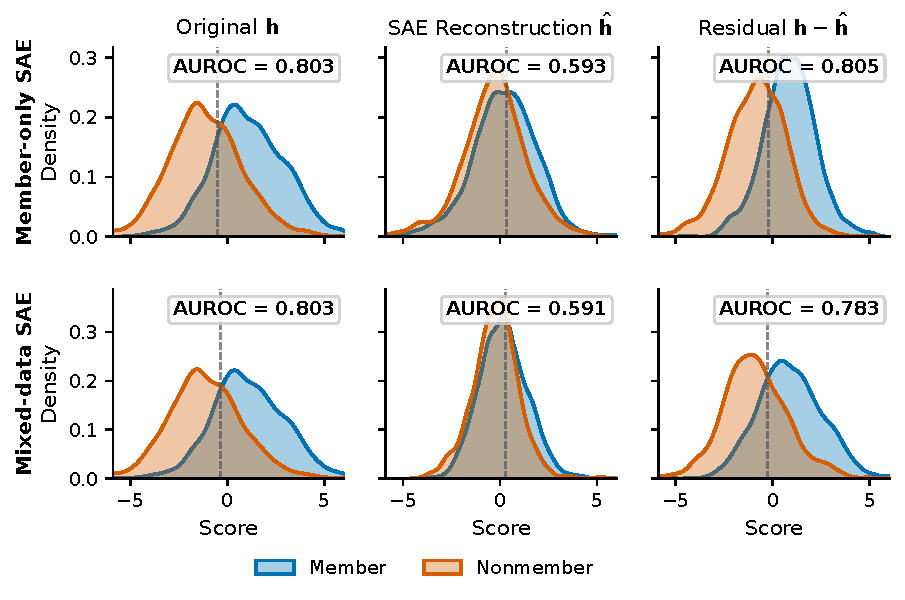
\includegraphics[width=\linewidth]{figures/score_distributions.pdf}
  \caption{Full score distribution comparison for Pythia-6.9B under both SAE types.
  \textbf{Top row} shows the member-only SAE. The center panel shows near-complete collapse of member--non-member separation (AUROC drops from 0.80 to 0.59).
  \textbf{Bottom row} shows the mixed-data SAE control. Separation still collapses (AUROC drops to 0.65), arguing against biased SAE training as the explanation.
  In both cases, probes recover the separation from the reconstruction residual (right panels).}
  \label{fig:score_distributions_full}
\end{figure}

\begin{figure}[tbp]
  \centering
  
\includegraphics[width=0.5\linewidth]{figures/sae_quality_vs_drop.pdf}
  \caption{SAE reconstruction quality (cosine similarity) versus membership AUROC drop.
  There is no significant correlation ($R^2 = 0.15$), suggesting that the reconstruction-induced drop is not simply an artifact of poor SAE reconstruction.
  GPT-Neo-2.7B achieves near-perfect reconstruction (cosine $= 0.998$) yet still loses 4 percentage points of membership detection, showing that reconstruction quality alone does not explain the effect.}
  \label{fig:sae_quality_scatter}
\end{figure}

\begin{table}[!htbp]
\centering
\caption{L2-normalized residual membership AUROC.
After normalizing residual vectors to unit length, all seven models retain the directional membership signal.
In three models with elevated residual norm AUROC (marked $^{*}$), L2 normalization increases the directional score, indicating that the norm effect partially masked directional signal.}
\label{tab:l2_normalized}
\appCompactTable{\begin{tabular}{@{}lcccc@{}}
\toprule
\textbf{Model} & \textbf{Raw Resid} & \textbf{L2 Resid} & \textbf{Norm Resid} & \textbf{$\Delta$(L2$-$Raw)} \\
\midrule
Pythia-1B      & 0.677 & 0.676 & 0.547 & $-$0.001 \\
GPT-Neo-2.7B   & 0.699 & 0.698 & 0.518 & $-$0.001 \\
Pythia-6.9B    & 0.805 & 0.806 & 0.511 & $+$0.001 \\
Mistral-7B     & 0.926 & 0.925 & 0.692 & $-$0.001 \\
OPT-6.7B$^{*}$     & 0.866 & 0.873 & 0.958 & $+$0.007 \\
Pythia-12B$^{*}$    & 0.814 & 0.831 & 0.995 & $+$0.017 \\
Qwen2-7B$^{*}$     & 0.849 & 0.858 & 0.982 & $+$0.009 \\
\bottomrule
\end{tabular}}
\end{table}

\begin{figure}[tbp]
  \centering
  
\includegraphics[width=\linewidth]{figures/norm_direction_decomposition.pdf}
  \caption{Norm versus directional contributions to membership detection by architecture family.
  GPT-family models rely almost entirely on directional structure (norm AUROC near chance at 0.51--0.60).
  LLaMA-family models encode membership in both magnitude and direction.
  Gap annotations show the directional contribution beyond norms.}
  \label{fig:norm_direction}
\end{figure}

\begin{figure}[tbp]
  \centering
  
\includegraphics[width=\linewidth]{figures/layer_heatmap.pdf}
  \caption{Membership detection AUROC across all layers for each model, normalized by model depth.
  Darker cells indicate stronger membership signal.
  The layer-wise concentration pattern differs by architecture family, with GPT-family models showing broad mid-layer activation and LLaMA-family models showing sharper peaks.}
  \label{fig:layer_heatmap}
\end{figure}

\FloatBarrier

\section{Robustness Checks and Boundary Conditions}
\label{app:robustness_boundary}

\subsection{Held-out Partition-Fit Probe for $\dK$}
\label{app:heldout_dk}

\begin{table*}[!htbp]
\centering
\caption{Per-split held-out drops from the partition-fit probe for $\dK$ (\S\ref{sec:methods:disclosures}).
Each split estimates $\dK$ on a random 70 percent of the canonical N=2000 labelled pool and evaluates the $\mathrm{score}_K$ drop on the disjoint 30 percent held-out partition.
Bootstrap CIs use $n_{\mathrm{boot}} = 10000$.
The column $\Delta_{\mathrm{HO-IP}}$ reports the per-split held-out drop minus the in-partition mean drop on the same model.}
\label{tab:heldout_dk_per_split}
\appWideTable{\begin{tabular}{@{}lccccc@{}}
\toprule
\textbf{Model} & \textbf{split\_seed} & \textbf{Held-out drop} & \textbf{95\% CI} & $\Delta_{\mathrm{HO-IP}}$ & \textbf{recon\_cos} \\
\midrule
\multicolumn{6}{@{}l}{\emph{Pythia-6.9B layer 16, seed 43, mult=4 L1=5e-4}} \\
P6.9B & 0 & 0.145 & {\scriptsize[0.106, 0.184]} & $-$0.068 & 0.979 \\
P6.9B & 1 & 0.171 & {\scriptsize[0.123, 0.220]} & $-$0.042 & 0.979 \\
P6.9B & 2 & 0.166 & {\scriptsize[0.123, 0.210]} & $-$0.047 & 0.979 \\
P6.9B & 3 & 0.199 & {\scriptsize[0.155, 0.243]} & $-$0.014 & 0.979 \\
P6.9B & 4 & 0.135 & {\scriptsize[0.088, 0.181]} & $-$0.078 & 0.979 \\
P6.9B & 5 & 0.158 & {\scriptsize[0.117, 0.201]} & $-$0.055 & 0.979 \\
P6.9B & 6 & 0.155 & {\scriptsize[0.113, 0.198]} & $-$0.058 & 0.979 \\
P6.9B & 7 & 0.149 & {\scriptsize[0.111, 0.187]} & $-$0.064 & 0.979 \\
P6.9B & 8 & 0.054 & {\scriptsize[0.012, 0.097]} & $-$0.159 & 0.979 \\
P6.9B & 9 & 0.157 & {\scriptsize[0.117, 0.197]} & $-$0.056 & 0.979 \\
\midrule
\multicolumn{6}{@{}l}{\emph{Pythia-12B layer 18, seed 49, mult=4 L1=5e-4}} \\
P12B & 0 & 0.106 & {\scriptsize[0.064, 0.148]} & $-$0.054 & 0.992 \\
P12B & 1 & 0.122 & {\scriptsize[0.074, 0.171]} & $-$0.038 & 0.992 \\
P12B & 2 & 0.129 & {\scriptsize[0.089, 0.171]} & $-$0.031 & 0.992 \\
P12B & 3 & 0.155 & {\scriptsize[0.112, 0.198]} & $-$0.005 & 0.992 \\
P12B & 4 & 0.104 & {\scriptsize[0.054, 0.153]} & $-$0.057 & 0.992 \\
P12B & 5 & 0.084 & {\scriptsize[0.040, 0.128]} & $-$0.077 & 0.992 \\
P12B & 6 & 0.110 & {\scriptsize[0.064, 0.157]} & $-$0.050 & 0.992 \\
P12B & 7 & 0.082 & {\scriptsize[0.043, 0.120]} & $-$0.078 & 0.992 \\
P12B & 8 & 0.042 & {\scriptsize[$-$0.004, 0.088]} & $-$0.119 & 0.992 \\
P12B & 9 & 0.120 & {\scriptsize[0.079, 0.161]} & $-$0.040 & 0.992 \\
\bottomrule
\end{tabular}}
\end{table*}

The Pythia-6.9B in-partition mean drop is 0.213, and the Pythia-12B in-partition mean drop is 0.160. Neither Pythia model meets the pre-specified magnitude criterion for the held-out drop, although the qualitative residual-over-reconstruction ordering is preserved.
The run record is \texttt{paper5/\allowbreak{}results/\allowbreak{}heldout\_\allowbreak{}dk\_\allowbreak{}2026-\allowbreak{}05-\allowbreak{}02.json}.

\subsection{Per-Row Bootstrap on the K-OC-2 Cohort}
\label{app:koc2_bootstrap}

\begin{table*}[!htbp]
\centering
\caption{Per-row paired bootstrap on the K-OC-2 cohort.
Margin is residual AUROC minus reconstruction AUROC.
CI bounds use $n_{\mathrm{boot}} = 10000$ and bootstrap seed 0.
Pseudo-replication on Qwen2-7B at multiplier 4 across two further fine-tune seeds (43 and 44) checks whether the inversion is seed-42-specific.
The K-OC-2 cohort overlaps with the main validity-passing set in Table~\ref{tab:dark_subspace} but is not identical, so this table is a related per-row direction-of-effect audit rather than the exact denominator of the binomial sign test reported in the main text.}
\label{tab:koc2_bootstrap_per_row}
\appWideTable{\begin{tabular}{@{}lcccccc@{}}
\toprule
\textbf{Row} & \textbf{Original} & \textbf{Recon} & \textbf{Residual} & \textbf{Margin} & \textbf{95\% CI} & \textbf{CI excl.\ 0} \\
\midrule
\multicolumn{7}{@{}l}{\emph{Controlled Pythia experiments}} \\
P6.9B N=5 seed 42 (postfix)        & 0.803 & 0.591 & 0.783 & $+$0.193 & {\scriptsize[$+$0.160, $+$0.227]} & yes \\
P12B fresh-init seed 47            & 0.764 & 0.596 & 0.726 & $+$0.130 & {\scriptsize[$+$0.094, $+$0.166]} & yes \\
\midrule
\multicolumn{7}{@{}l}{\emph{Cross-architecture sweep}} \\
P1B mult=4 layer 14 seed 42        & 0.663 & 0.592 & 0.671 & $+$0.079 & {\scriptsize[$+$0.060, $+$0.099]} & yes \\
P2.8B mult=4 layer 20 seed 42      & 0.799 & 0.683 & 0.803 & $+$0.120 & {\scriptsize[$+$0.098, $+$0.142]} & yes \\
Qwen2-7B mult=4 seed 42            & 0.638 & 0.553 & 0.673 & $+$0.120 & {\scriptsize[$+$0.086, $+$0.153]} & yes \\
Qwen2-7B mult=8 seed 42            & 0.638 & 0.552 & 0.674 & $+$0.122 & {\scriptsize[$+$0.090, $+$0.153]} & yes \\
GPT-Neo-2.7B mult=8 seed 42        & 0.616 & 0.580 & 0.652 & $+$0.072 & {\scriptsize[$+$0.049, $+$0.095]} & yes \\
\midrule
\multicolumn{7}{@{}l}{\emph{Qwen2-7B mult=4 pseudo-replication}} \\
Qwen2-7B mult=4 seed 43 (secondary) & 0.638 & 0.585 & 0.658 & $+$0.073 & {\scriptsize[$+$0.050, $+$0.096]} & yes \\
Qwen2-7B mult=4 seed 44 (secondary) & 0.638 & 0.578 & 0.659 & $+$0.081 & {\scriptsize[$+$0.056, $+$0.106]} & yes \\
\bottomrule
\end{tabular}}
\end{table*}

The run record is \texttt{paper5/\allowbreak{}results/\allowbreak{}k\_\allowbreak{}oc2\_\allowbreak{}bootstrap\_\allowbreak{}residual\_\allowbreak{}minus\_\allowbreak{}reconstruction\_\allowbreak{}2026-\allowbreak{}05-\allowbreak{}05.json}.

Every row in this cohort has residual AUROC above reconstruction AUROC with the 95 percent CI excluding zero, consistent with the residual-over-reconstruction ordering reported in the main text.

\subsection{Bag-of-Words Vocabulary Baseline}
\label{app:bow_baseline}

A natural concern is that the residual detector might be detecting surface vocabulary rather than internal model structure. We test that explanation directly with a unigram bag-of-words classifier on the same 1000 member and 1000 non-member documents used for the controlled Pythia-6.9B reconstruction/residual evaluation. The classifier is a logistic regression trained on CountVectorizer word-count features with five-fold stratified cross-validation, and AUROC is computed after pooling the out-of-fold predictions.

The pooled AUROC is 0.4566, rounded to 0.457 in Table~\ref{tab:dark_subspace}, so this token-level baseline does not distinguish members from non-members on the controlled split. The result argues against a simple unigram vocabulary account of the residual signal. It does not rule out higher-order surface artefacts, since the bag-of-words representation discards word order and context. The numerical record is \texttt{runs/\allowbreak{}memcirc/\allowbreak{}bow\_\allowbreak{}ceiling/\allowbreak{}memcirc\_\allowbreak{}ctrl\_\allowbreak{}ft/\allowbreak{}results.json}.

\subsection{Per-Model SAE Hyperparameter Detail}
\label{app:per_model_hps_detail}

\paragraph{Dictionary form.}
We use ReLU plus L1 dictionaries to match the prior SAE-based memorisation work we audit~\citep{wang2025sspu,frikha2025privacyscalpel,muhamed2025dsg,suri2025mitigating}. The reconstruction/residual decomposition itself requires only a learned decoder dictionary $W_{\mathrm{dec}}$, but all main interpretations are conditioned on adequate reconstruction fidelity, following the SAEBench emphasis on reconstruction quality as a prerequisite for feature-level interpretation~\citep{karvonen2025saebench}. JumpReLU, TopK, BatchTopK, and Matryoshka SAE replications are future work.

Table~\ref{tab:per_model_hps} records the SAE settings used for the main decomposition rows. Hyperparameters are chosen to obtain an interpretable reconstruction under the reconstruction-quality criterion in \S\ref{sec:methods:disclosures}, not to maximise the reconstruction-induced drop. For each model we tune the dictionary expansion ratio and the L1 sparsity coefficient, requiring reconstruction cosine at least 0.90 and mean L0 below 60\% of dictionary size for the strict rows. The Pythia-6.9B mixed-data SAE uses the corrected five-seed mixed-data run at mult=4 and L1=5e-4.

Pythia-6.9B and Pythia-12B both use mult=4 and L1=5e-4. Qwen2-7B and GPT-Neo-2.7B require mult=8 to clear the strict reconstruction criterion. OPT-6.7B clears at mult=8 with L1=2e-4 and is included only for residual norm decomposition, since its residual carries norm signal independently of direction (Table~\ref{tab:l2_normalized}). Mistral-7B does not reconstruct activations reliably enough under the plain-L1 configurations we swept. The mixed-data SAE configurations are recorded in the per-seed \texttt{config.json} files under \texttt{runs/\allowbreak{}memcirc/\allowbreak{}sae\_\allowbreak{}dark\_\allowbreak{}subspace/\allowbreak{}<model>\_\allowbreak{}mixed\_\allowbreak{}sae*}, with the wider retuning and unsuccessful attempts documented in Appendix~\ref{app:qwen2_pilot}.

\begin{table*}[!htbp]
\centering
\caption{Per-model sparse autoencoder hyperparameters under the reconstruction-quality criterion.
The dictionary expansion ratio and L1 coefficient are the two main settings.
The Pythia-6.9B row reports the corrected mixed-data five-seed recipe (mult=4, L1=5e-4).
The Mistral-7B row reports the L1 range swept across plain-L1 attempts, all of which fall under threshold failure.
The elastic-net sweep referenced in the limitations is documented separately in Appendix~\ref{app:qwen2_pilot}.}
\label{tab:per_model_hps}
\appWideTable{\begin{tabular}{@{}llcc@{}}
\toprule
\textbf{Model} & \textbf{Status} & \textbf{Ratio} & \textbf{L1} \\
\midrule
Pythia-6.9B    & passes threshold                  & 4 & $5\mathrm{e}{-4}$ \\
Pythia-12B     & passes threshold (replication)    & 4 & $5\mathrm{e}{-4}$ \\
Qwen2-7B       & passes threshold at mult 8        & 8 & $5\mathrm{e}{-4}$ \\
GPT-Neo-2.7B   & passes threshold at mult 8        & 8 & $5\mathrm{e}{-4}$ \\
Pythia-1B      & wider band (cross-arch only)      & 4 & $5\mathrm{e}{-4}$ \\
Pythia-2.8B    & wider band (cross-arch only)      & 4 & $5\mathrm{e}{-4}$ \\
Falcon-7B      & sparsity boundary (cross-arch)    & 4 & $5\mathrm{e}{-4}$ \\
OPT-6.7B       & residual norm confound            & 8 & $2\mathrm{e}{-4}$ \\
Mistral-7B     & threshold failure (L1 sweep)      & 4 & 1$\mathrm{e}{-4}$ to 5$\mathrm{e}{-4}$ \\
Llama-3-8B     & failed reconstruction criterion   & 4 & $5\mathrm{e}{-4}$ \\
\bottomrule
\end{tabular}}
\end{table*}

The hyperparameter retuning is per-model. The reconstruction/residual result is therefore conditional on each model's reliable-reconstruction configuration, not a fixed-hyperparameter comparison. Cross-model replication across JumpReLU, TopK, BatchTopK, and Matryoshka SAEs remains future work.

\subsection{L1-regularized SAE Training Instability}
\label{app:sae_l1_instability}

Standard L1-regularized ReLU SAE training is sensitive to random initialization near the sparsity phase transition~\citep{bricken2023monosemanticity}. Below the transition, training collapses into a dense basin where most features fire on most tokens. Above the transition, training reaches a sparse basin with the target mean L0. The transition L1 depends on activation magnitude statistics that vary across model and layer, so a single global L1 cannot guarantee sparse-basin convergence on every model.

We observe this empirically in supplementary five-seed retraining checks on the cross-architecture SAEs at L1 $= 5 \times 10^{-4}$. The controlled Pythia experiments at this same L1 train into the sparse basin on every seed (mean L0 below 2 percent of dictionary size across the three configurations, reconstruction cosine above $0.92$). On GPT-Neo-2.7B with the same hyperparameter, two of five retrained seeds reach the sparse basin (mean L0 near $700$ of $20480$ features, reconstruction cosine $0.998$). The remaining seeds collapse into the dense basin (mean L0 near $17000$ of $20480$, reconstruction cosine between $0.16$ and $0.60$). The two outcomes are not noisy estimates of a single result. They are distinct training basins, consistent with the documented L1 phase transition and with the SAE-quality conventions reviewed by~\citet{karvonen2025saebench}.

The validity gate handles this failure mode by construction. Dense-basin training runs fall well below both the $0.85$ permissive and the $0.90$ strict reconstruction-cosine thresholds and are excluded from quantitative comparison. Newer SAE variants such as TopK~\citep{gao2025scaling} and BatchTopK~\citep{bussmann2024batchtopk} avoid the L1 transition by replacing the sparsity penalty with a hard top-$k$ selection, but this paper deliberately scopes to the standard L1-regularized ReLU recipe used by the membership-related interventions we audit.

\subsection{Held-Out Partition-Fit Probe Protocol}
\label{app:heldout_dk_protocol}

We test whether the single score$_K$ direction depends on the partition used to estimate it by re-fitting $\dK$ on one labeled split and evaluating it on the held-out split (\S\ref{sec:methods:disclosures}).

A separate concern is whether the membership direction $\dK$ is tied to the labelled partition used to fit it. If the direction shifts across partitions, the precise $\mathrm{score}_K$ drop in Table~\ref{tab:dark_subspace} should be read as partition-conditional even if the residual-over-reconstruction ordering still holds.

We test this by splitting the canonical 2000-document labelled pool into a 70\% subset for fitting $\dK$ and a disjoint 30\% subset for evaluation. Pythia-6.9B uses layer 16 from the seed 43 mult=4 L1=5e-4 SAE, and Pythia-12B uses layer 18 from the seed 49 mult=4 L1=5e-4 SAE. For each of ten random splits, we re-fit $\dK$ on the fitting subset, evaluate $\mathrm{score}_K$ AUROC on the held-out subset, and compute the held-out reconstruction drop with 10000 bootstrap resamples. The stability threshold compares the held-out drop against the in-partition drop minus two cross-split standard deviations.

The magnitude claim does not pass this stability check. On Pythia-6.9B, the in-partition mean drop is 0.213 with cross-split standard deviation 0.012, while the mean held-out drop is 0.149. On Pythia-12B, the in-partition mean drop is 0.160 with cross-split standard deviation 0.012, while the mean held-out drop is 0.105. In both cases, the held-out drop falls below the corresponding threshold. The qualitative residual-over-reconstruction ordering nevertheless survives held-out estimation on both Pythia models. This probe therefore narrows the quantitative claim without overturning the qualitative decomposition result. Per-split numerical detail is recorded in \texttt{paper5/\allowbreak{}results/\allowbreak{}heldout\_\allowbreak{}dk\_\allowbreak{}2026-\allowbreak{}05-\allowbreak{}02.json} and Table~\ref{tab:heldout_dk_per_split}.

\subsection{Pythia-12B Replication Detail}
\label{app:p12b_replication}

Pythia-12B asks whether the controlled Pythia-6.9B finding recurs at larger scale within the same model family. We train five independent mixed-data SAEs on Pythia-12B layer 18 at mult=4 and L1=5e-4 under the corrected training pipeline. The retained seeds are 47 through 51, each with an isolated output directory. An earlier array using seeds 42 through 46 collided into two output directories because the task identifier was missing from the directory name, so those evaluations are superseded.

All five retained SAEs clear the reconstruction criterion, with reconstruction cosine in $[0.991, 0.992]$. The reconstruction drops are 0.169, 0.139, 0.160, 0.131, and 0.161, giving mean 0.152 and standard deviation 0.016. Each drop is above the 0.10 strong-effect threshold. The residual AUROC sits below the original on all five evaluations, but it is more stable across seeds than the dictionary projection. Residual AUROC standard deviation is 0.005, while dictionary-projection AUROC standard deviation is 0.016. Since the original AUROC is fixed at 0.764, the drop variance is the dictionary-projection variance by construction.

This replication varies SAE initialization while holding the fine-tuned Pythia-12B model fixed. It therefore supports a within-family scale replication of the residual-over-reconstruction pattern, but it does not characterize fine-tuning-seed variance at 12B and does not establish cross-architecture controlled replication. Per-seed records are in \texttt{runs/\allowbreak{}memcirc/\allowbreak{}sae\_\allowbreak{}dark\_\allowbreak{}subspace/\allowbreak{}p12b\_\allowbreak{}mixed\_\allowbreak{}sae\_\allowbreak{}seed\{47..51\}/\allowbreak{}results.json}.

\subsection{Gemma-2-2B Stretch Experiment}
\label{app:gemma_stretch}

Gemma-2-2B adds a Google-family model to the qualitative architecture sweep. We train one mixed-data SAE at layer 16 with multiplier 4 ($d_{\text{sae}} = 9{,}216$) and L1 = 5e-4 on the union of 1000 member and 1000 non-member OpenWebText activations, then evaluate the same reconstruction/residual decomposition on the canonical evaluation pool. The run uses one fine-tuning seed and one SAE seed.

The reconstruction cosine is 0.911, and the mean number of active features is 1408.6 out of 9216. Original $\mathrm{score}_K$ AUROC is 0.801, SAE-reconstruction AUROC is 0.769, and residual AUROC is 0.820. The reconstruction drop is only 0.032, below the 0.10 strong-effect threshold used for the controlled Pythia claim, but the qualitative ordering residual $>$ original $>$ reconstruction holds. The residual norm AUROC is 0.612, below the 0.65 norm-confound flag. Gemma also satisfies the residual-over-reconstruction ordering at this single seed, consistent with the binomial sign test reported in the main results section.

Gemma-2-2B therefore contributes to qualitative generality, not to the within-model strong-drop evidence. The model is smaller than the controlled Pythia experiments, and neither fine-tuning-seed variance nor SAE-seed variance is characterized here. The run record is \texttt{runs/\allowbreak{}memcirc/\allowbreak{}sae\_\allowbreak{}dark\_\allowbreak{}subspace/\allowbreak{}gemma2\_\allowbreak{}2b\_\allowbreak{}mixed\_\allowbreak{}sae/\allowbreak{}results.json}.

\paragraph{Sparsity scope of the geometric and feature-alignment analyses.}
The full BCD, FSC, norm-direction, and layer-trajectory analyses were extended to Gemma-2-2B in a follow-up run that landed on 2026-05-05. The Gemma SAE used for these analyses operates at mean $L_0$ of 1408 of 9216 features (15.3 percent), substantially above the comparable range across the other rows in Table~\ref{tab:dark_subspace}, namely Pythia-12B at 0.05 percent, Qwen2-7B with multiplier 8 at 0.01 percent, Pythia-1B at 1.29 percent, Pythia-6.9B at 1.68 percent, and GPT-Neo-2.7B with multiplier 8 at 3.77 percent. The reconstruction cosine remains within the validity gate at 0.911, so the residual signal in Table~\ref{tab:dark_subspace} is comparable in that gate's terms. The disparity arises because the same L1 coefficient ($5 \times 10^{-4}$) does not equally constrain activation magnitudes across model families, and Gemma's activations require a stronger penalty to reach the standard sparsity range.

We split the Gemma full-analyses into four findings by their dependence on SAE feature sparsity. The residual-over-reconstruction ordering (Table~\ref{tab:dark_subspace}) depends only on reconstruction cosine, which Gemma satisfies, so this finding stands without sparsity scoping. The BCD double-dissociation min principal angle of 38.33 degrees, against the typical 75 degrees and above on the other models, is computed from raw activations through contrastive principal component analysis without any SAE involvement, so this finding is also independent of the sparsity disparity. The norm-direction membership AUROC of 0.600 at the best layer is a pure activation-magnitude analysis with no SAE dependence and is also independent of sparsity. The feature-alignment asymmetry $\mathrm{FSC}_K^{\mathrm{cf}}$ approximately equal to $\mathrm{FSC}_R^{\mathrm{cf}}$ (0.414 against 0.425) on Gemma, however, depends directly on which SAE features are classified as content-familiar and how selective those features are. At a near-dense $L_0$ of 15.3 percent, feature selectivity is materially weaker than at sub-4-percent $L_0$, and the asymmetry observed on the other rows requires sparse selective features to manifest. We therefore restrict the analyses in Tables~\ref{tab:bcd_main}, \ref{tab:norm_direction}, and \ref{tab:fsc_values} and Figure~\ref{fig:layer_trajectories} to the SAE settings within the comparable sparsity range. Gemma is retained in Table~\ref{tab:dark_subspace} where the validity gate is satisfied. The BCD geometric measurement and the norm-direction measurement for Gemma are reported in this appendix for completeness, and are not integrated into the main geometric tables. A retrain at stronger L1 is in progress, and if it converges to $L_0$ within the standard range while the geometric and feature-alignment analyses then match the other rows, the paper will be updated to integrate Gemma fully.

\subsection{Standard Probe Replication and Output-Layer Scope}
\label{app:standard_probes}

The main text scopes the reconstruction/residual result to a layer-local measurement. This entry explains why. A natural alternative reading is that the effect reflects the $\mathrm{score}_K$ probe rather than the internal representation. To test this, we repeat the SAE patching decomposition on Pythia-6.9B fine-tuned for 5 epochs with three standard membership inference probes. The probes are the loss attack, MIN-K\%=20, and zlib, following the canonical implementations referenced in \citet{yeom2018privacy}, \citet{shi2023detecting}, and \citet{carlini2021extracting}. Probe outputs are recorded in \texttt{runs/\allowbreak{}memcirc/\allowbreak{}standard\_\allowbreak{}mia\_\allowbreak{}probes/\allowbreak{}p69\_\allowbreak{}dark\_\allowbreak{}subspace\_\allowbreak{}replication/\allowbreak{}results.json}.

For each probe we compare original AUROC on raw activations, AUROC after SAE reconstruction, and AUROC on the residual. The replication criterion requires the reconstruction AUROC to drop by at least 0.05 on at least two of the three probes. It is not met. The original AUROC saturates on all three probes, and the SAE-patched reconstruction AUROC stays within rounding of the original. This result suggests that downstream layers and the LM head compensate for the SAE-patched activation. The reconstruction drop is therefore a property of the layer-local internal measurement, not an output-level improvement to standard membership attacks.

\paragraph{Direction estimation and bootstrap conventions.}
The membership direction $\dK$ used for $\mathrm{score}_K$ is fitted by five-fold cross-validation on the OpenWebText evaluation partition, with the projection then computed on held-out folds. All AUROC and $\Delta$AUROC confidence intervals reported in the body and appendix tables use $n_{\mathrm{boot}} = 10{,}000$ paired bootstrap resamples, with bootstrap pairs at the document level so that the same labelled rows enter the resample on the original and the comparison condition. Standard deviation across SAE seeds is reported separately from the bootstrap interval where independently trained SAEs are compared, since seed variance and within-fit variance answer different questions.

\subsection{Detailed Limitations and Boundary Conditions}
\label{app:limitations_detail}

The main text states the claim boundaries compactly. This entry expands them so that each limitation can be read against the claim it bounds.

\paragraph{Held-out partition sensitivity of the magnitude claim.}
Held-out estimation of $\dK$ supports the qualitative residual-over-reconstruction ordering but not the original magnitude claim. Re-fitting $\dK$ on a 70 percent partition and evaluating on a disjoint 30 percent partition produces a smaller mean reconstruction-induced drop than the in-partition value (Pythia-6.9B in-partition 0.213 against held-out 0.149; Pythia-12B in-partition 0.160 against held-out 0.105). The qualitative residual $\geq$ original $>$ reconstruction ordering nevertheless survives held-out estimation on both Pythia models. The interpretation is therefore split. $\dK$ as a single direction is partition-sensitive in magnitude, and the residual-over-reconstruction ordering is not driven by evaluating and fitting that direction on the same documents.

\paragraph{SAE variant scope.}
The SAE conclusion is limited to standard L1-regularized ReLU SAEs as evaluated here. Newer variants such as JumpReLU, TopK, BatchTopK, and Matryoshka SAEs alter the reconstruction and sparsity tradeoff, so they should be audited before generalizing the result to all sparse dictionary parameterizations~\citep{rajamanoharan2024jumping,gao2025scaling,bussmann2024batchtopk,bussmann2025matryoshka}.

\paragraph{Practical implication.}
The detection-extraction dissociation and the paraphrase-orientation diagnostic together support a single practical conclusion. SAE feature-level editing should not be treated as a privacy guarantee unless the target model is audited for membership signal recoverable from the reconstruction residual.

We separate two evidence sources. The controlled Pythia experiments carry the primary causal evidence, because both the member-only and mixed-data dictionaries reproduce the same residual-over-reconstruction ordering at reconstruction quality that passes the validity gate. The cross-architecture sweep across non-Pythia models provides corroborating evidence where reconstruction quality is sufficient, and is reported as a diagnostic where it is not. This sweep supports qualitative generality of the residual-over-reconstruction ordering, not a universal architecture-level law. The norm-direction split across architecture families is descriptive. The residual-PC ablation suggests partial low-dimensional structure, yet it does not satisfy the stronger falsification criteria needed for causal localization. These findings concern layer-local membership recoverability under controlled fine-tuning with IID member and non-member splits, not individual-sentence pre-training MIA, which recent work has shown to be largely confounded by distribution shift~\citep{maini2024dataset, duan2024membership}. The fine-tuning regime amplifies per-sample membership signal beyond what is observable at pre-training scale.

The strongest causal evidence is within Pythia. The matched-hyperparameter mixed-data SAE control succeeds on Pythia-6.9B, and Pythia-12B provides a within-family replication at smaller magnitude. Replication attempts on GPT-Neo-2.7B across five L1 settings and Mistral-7B across two L1 settings did not reconstruct activations reliably enough for controlled decomposition evidence (Appendix~\ref{app:qwen2_pilot}). The broader cross-architecture pattern supports qualitative generality, but it is not the same kind of controlled replication as the Pythia experiments.

All nine models share the same fine-tuning protocol and the same OpenWebText member partition. This design controls the document unit and distribution matching, but it also means that any artifact of the shared fine-tuning setup could affect both the controlled and descriptive results. The Pythia-6.9B corpus-disjointness check argues against SAE train-test corpus overlap on that model (\S\ref{sec:methods:disclosures}), but cross-corpus replication for the remaining models is future work.

Several model-specific outcomes define scope rather than contradicting the main result. Llama-3-8B did not reconstruct activations reliably enough under the attempted configuration. The Qwen2-7B mixed-data pilot fell below the strict reconstruction-cosine threshold at multiplier 4, while the multiplier-8 retune clears the threshold and enters the cross-architecture set. A Mistral-7B elastic-net SAE sweep across three $\lambda_{L_2}$ settings did not yield an interpretable reconstruction, so Mistral is excluded from the cross-model set. The family pattern reported descriptively in \S\ref{sec:results:controls} therefore comprises Pythia-6.9B, Pythia-12B, GPT-Neo-2.7B, and Qwen2-7B.

The single $\mathrm{score}_K$ direction is partition-sensitive. The held-out estimation probe (\S\ref{sec:results:dark}) shows that the magnitude of the $\mathrm{score}_K$ drop is reduced when $\dK$ is fit and evaluated on disjoint label partitions. The qualitative residual-over-reconstruction ordering is preserved on held-out partitions at both Pythia models, so the residual-recoverability finding is partition-fit-independent at the qualitative level. The precise drop magnitudes are not.

The privacy-aware SAE experiment covers two models, and post-unlearning persistence is not tested. These limitations interact. A reviewer evaluating any one boundary should read it together with the others, since the claim depends on the access setting, corpus, SAE family, and evidence tier.

\subsection{Additional Controls}
\label{app:additional_controls}

The controls paragraph in \S\ref{sec:results:controls} groups several checks by the alternative explanations they address. This entry gives the per-control method and outcome. Per-control numerical detail is recorded under \texttt{runs/memcirc/}, with seeds and configs documented in each run's \texttt{config.json}.

The pre-fine-tuning negative control asks whether the membership direction exists before fine-tuning. Re-running the channel detector on the un-fine-tuned base Pythia-6.9B model across the same five layers leaves the detector at chance, so the membership signal requires fine-tuning. The layer sensitivity sweep asks whether layer 16 was chosen because it was unusually favourable. Re-running the membership detector on layers 12, 14, 16, 18, and 20 shows that AUROC increases monotonically with depth, while $\dK$ and $\dR$ remain near-orthogonal across the swept layers.

The random-direction baseline asks whether arbitrary residual-stream directions can separate members from non-members. For each model, we draw 100 random unit directions and compute membership AUROC. The fixed-orientation random-direction mean sits near chance on every model, and the 99th percentile remains below the fitted membership direction. The random-init SAE control asks whether the result follows from any reconstruction-shaped operator. Replacing the trained SAE on Pythia-6.9B layer 16 with a randomly initialised SAE collapses reconstruction cosine to near zero and drops reconstructed $\mathrm{score}_K$ AUROC to chance. The trained SAE reaches near-unity reconstruction cosine yet still drops reconstructed AUROC, indicating that the finding requires a learned high-fidelity dictionary.

The GPT-Neo-2.7B multiplier-8 pilot and Qwen2-7B multiplier-8 retune test whether denser dictionaries change the qualitative ordering. GPT-Neo-2.7B reconstructs almost perfectly and reproduces the residual-greater-than-original inversion at lower magnitude, with $\dK$ coverage cosine near zero. Qwen2-7B clears the strict reconstruction-cosine threshold at multiplier 8. Its drop magnitude increases relative to multiplier 4 but remains below the strong-effect threshold, while $\dK$ coverage cosine increases substantially. The Qwen2 retune is therefore reported as an SAE-quality improvement for Qwen2, not as a non-Pythia strong-drop result. The random-init SAE control remains Pythia-6.9B only.

The Pythia-12B $K=10$ ablation in Table~\ref{tab:kpc_kten_cells} uses the member-only SAE for continuity with the Pythia-6.9B configuration. We also rerun the same ablation on the Pythia-12B mixed-data SAE used for the reconstruction/residual evaluation, using seed 47 and leaving the remaining settings unchanged. The rerun is recorded at \texttt{runs/\allowbreak{}memcirc/\allowbreak{}causal\_\allowbreak{}ablation/\allowbreak{}p12b\_\allowbreak{}errPC\_\allowbreak{}K10\_\allowbreak{}schemaA\_\allowbreak{}seed47/\allowbreak{}}.

The mixed-data rerun reduces the ablation effect from $+0.176$ in the body cell to $+0.018$ (95\% CI $[0.015, 0.022]$). The matched-Gaussian-noise control produces a larger drop than the targeted subspace, and the random 5\% column-mask control reproduces the ablated AUROC. Reconstruction cosine is 0.991. The per-text residual-to-original-norm ratio is 0.308 and is recorded as a script-level sanity-check failure, but this ratio is not part of the pre-registered reconstruction and sparsity criteria.

This outcome is why the subspace ablation is treated as illustrative rather than as the reference point. It is consistent with residual membership signal being partially concentrated, but it does not pass the same-SAE and random-mask checks needed for a strong causal localization claim. The Pythia-12B mixed-data reconstruction/residual decomposition itself is unaffected, since that evaluation always used the mixed-data SAE array and reports a mean reconstruction drop of 0.152.

\begin{table}[!htbp]
\centering
\caption{Top-$K$ residual principal-component ablation on the four models that pass the reconstruction-quality criterion, at $K=10$ with $K=5$ as a sparser-support control.
The drop is the paired difference between the unablated and ablated probe AUROC, with bootstrap 95\% CI from 10000 resamples.
The pre-registered decisive criterion, where the primary intervention beats both random-rotation and matched-Gaussian noise controls at the 95\% bootstrap margin, is met on zero of the six cells.
Pythia-12B is the only model where $K=10$ produces a substantial subspace-level drop. The remaining cells sit at the floor.}
\label{tab:kpc_kten_cells}
\appCompactTable{\begin{tabular}{@{}llccc@{}}
\toprule
\textbf{Model} & \textbf{$K$} & \textbf{Drop} & \textbf{95\% CI} & \textbf{Decisive gate} \\
\midrule
Pythia-12B    & 10 & $+$0.176  & {\scriptsize[$+$0.165, $+$0.187]} & not met \\
Pythia-6.9B   & 10 & $+$0.025  & {\scriptsize[$+$0.021, $+$0.029]} & not met \\
Qwen2-7B      & 10 & $+$0.003  & {\scriptsize[$+$0.001, $+$0.005]} & not met \\
GPT-Neo-2.7B  & 10 & $-$0.001  & {\scriptsize[$-$0.004, $+$0.002]} & not met \\
\midrule
Pythia-12B    & 5  & $+$0.103  & {\scriptsize[$+$0.094, $+$0.112]} & not met \\
Pythia-6.9B   & 5  & $+$0.013  & ---                                & not met \\
Qwen2-7B      & 5  & $+$0.002  & ---                                & not met \\
GPT-Neo-2.7B  & 5  & $-$0.001  & ---                                & not met \\
\bottomrule
\end{tabular}}
\end{table}

A same-SAE rerun on the Pythia-12B mixed-data SAE collapses the $K=10$ row to $+0.018$. See Appendix~\ref{app:additional_controls}.

\subsection{Corpus-Disjoint Dictionary Control}
\label{app:corpus_disjoint}

The body controls paragraph uses this check to address train-test SAE corpus overlap on Pythia-6.9B. The concern is specific. The standard mixed-data SAE training pool overlaps with the canonical evaluation pool by construction, so the reconstruction drop could in principle reflect the SAE having seen evaluation documents during dictionary training.

To test that explanation, we retrain the Pythia-6.9B mixed-data SAE at the analysis layer on an OpenWebText partition selected to have zero document overlap with the reconstruction/residual evaluation pool. The multiplier, L1 coefficient, corrected corpus-cycling pipeline, fine-tuned model, and evaluation pool are held constant relative to the standard mixed-data run. The disjoint-corpus SAE configuration and per-document partition manifests are recorded under \texttt{runs/\allowbreak{}memcirc/\allowbreak{}sae\_\allowbreak{}dark\_\allowbreak{}subspace/\allowbreak{}p69\_\allowbreak{}disjoint\_\allowbreak{}corpus\_\allowbreak{}sae/\allowbreak{}}, with the document-overlap audit recorded alongside.

The disjoint-corpus dictionary clears the strict reconstruction criterion and yields a reconstruction drop in the favourable direction relative to the in-corpus baseline, marginally larger than the standard mixed-data dictionary under the same hyperparameter setting. The qualitative residual-over-reconstruction ordering is preserved. This argues against train-test SAE corpus contamination as the explanation on Pythia-6.9B. Cross-architecture replication of corpus-disjoint dictionary training remains future work.

\subsection{TPR at Low FPR and Paraphrase Diagnostic}
\label{app:tpr_paraphrase}

A bidirectional audit that picks the orientation maximizing AUROC on each evaluation condition is no longer a robustness test, because it lets the detector re-fit at evaluation time. A bidirectional report would conceal the orientation flip and inflate apparent paraphrase robustness, which is why the body §4.6 finding requires fixed-orientation AUROC.

The controls paragraph routes two privacy-audit details here. The first is whether the residual channel adds signal at low false-positive rates, where false accusations of training-data use are costly. The second is whether bidirectional AUROC reporting can obscure detector-direction sensitivity under paraphrase.

For the low-FPR audit, we measure the standard loss attack, zlib, and MIN-K\% baselines plus the residual $\dK$ channel at the 1\% FPR and 0.1\% FPR thresholds on Pythia-6.9B, Qwen2-7B, GPT-Neo-2.7B, and Pythia-12B at epoch 5. Controlled fine-tuning saturates per-example loss on three of the four models. On Pythia-6.9B, Qwen2-7B, and Pythia-12B, the standard loss, zlib, and Min-K-style baselines all reach the TPR ceiling at 1\% FPR. GPT-Neo-2.7B is the one model where loss does not saturate, and there the residual $\dK$ channel exceeds the best standard baseline with paired bootstrap CI above zero. At the stricter 0.1\% FPR threshold favoured for privacy-auditing evaluations~\citep{chen2026wbc, ilic2026ezmia}, the residual $\dK$ channel exceeds the original $\dK$ on three of four models, mirroring the AUROC-level pattern.

For the paraphrase diagnostic, we evaluate the SAE residual membership detector on word-order-shuffled paraphrases of member documents. We run the check first on Pythia-6.9B seed 42 and then replicate it on Qwen2-7B and Pythia-12B. A bidirectional AUROC helper reports a lift on paraphrases relative to originals, but the fixed-orientation audit shows that the detector direction flips between conditions. Under the orientation learned on originals, paraphrased member scores shift in the opposite direction relative to non-members. The paraphrased member and non-member distributions remain linearly separable, but in the reversed direction. We therefore treat the paraphrase outcome as a methodological warning about bidirectional AUROC reporting, not as evidence that paraphrasing increases memorisation. Per-run JSONs are under \texttt{runs/\allowbreak{}memcirc/\allowbreak{}tpr\_\allowbreak{}low\_\allowbreak{}fpr/\allowbreak{}} and \texttt{runs/\allowbreak{}memcirc/\allowbreak{}paraphrase\_\allowbreak{}probe/\allowbreak{}}.

\paragraph{Bidirectional AUROC and the reconstruction-residual comparison.}
The reconstruction-residual comparison in Table~\ref{tab:dark_subspace} uses the same bidirectional helper. Because that helper reports the larger of the two possible sign conventions on each view, a reader could reasonably ask whether the residual column scores high simply because the helper is allowed to flip the detector direction view by view. We checked this directly on every row with per-text scores on disk. The fitted membership direction separates members from non-members in the same way on the original activation, on the reconstruction, and on the residual. Members score higher than non-members on all three views, and no row ever requires the helper to swap signs. The reported values therefore match what a fixed-direction audit would have produced, so the residual-over-reconstruction ordering is a property of the activations themselves, not an artifact of giving the AUROC computation freedom to flip its sign. This is the opposite pattern from the paraphrase case above, where the orientation genuinely reverses and the bidirectional helper would hide that reversal.

\FloatBarrier

\section*{Code Availability}

Code, data, and analysis scripts are available at the repository associated with this submission. The repository structure and per-claim artefact mapping are documented in the artefact README at the repository root, and the pre-registration of the experimental protocol is in the accompanying pre-registration document. For initial submission this URL is suppressed for double-blind review. The URL is supplied at camera-ready stage.